%Dokumentklasse
\documentclass[a4paper,12pt]{scrreprt}
\usepackage[left= 2.5cm,right = 2cm, bottom = 4 cm]{geometry}
%\usepackage[onehalfspacing]{setspace}
% ============= Packages =============

% Dokumentinformationen
\usepackage[
	pdftitle={Titel der Abschlussarbeit},
	pdfsubject={},
	pdfauthor={Name},
	pdfkeywords={},	
	%Links nicht einrahmen
	hidelinks
]{hyperref}


% Standard Packages
\usepackage[utf8]{inputenc}
\usepackage[ngerman]{babel}
\usepackage[T1]{fontenc}
\usepackage{graphicx, subfig}
\graphicspath{{img/}}
\usepackage{fancyhdr}
\usepackage{lmodern}
\usepackage{color}

% zusätzliche Schriftzeichen der American Mathematical Society
\usepackage{amsfonts}
\usepackage{amsmath}

%nicht einrücken nach Absatz
%\setlength{\parindent}{0pt}


% ============= Kopf- und Fußzeile =============
\pagestyle{fancy}
%
\lhead{}
\chead{}
\rhead{\slshape \leftmark}
%%
\lfoot{}
\cfoot{\thepage}
\rfoot{}
%%
\renewcommand{\headrulewidth}{0.4pt}
\renewcommand{\footrulewidth}{0pt}

% ============= Package Einstellungen & Sonstiges ============= 
%Besondere Trennungen
\hyphenation{De-zi-mal-tren-nung}


% ============= Dokumentbeginn =============

\begin{document}
%Seiten ohne Kopf- und Fußzeile sowie Seitenzahl
\pagestyle{empty}

\begin{center}
\begin{tabular}{p{\textwidth}}


\begin{center}

\includegraphics[scale=0.5]{img/logos.jpg}
\end{center}
\\
\begin{center}
\LARGE{\textsc{
NDT PROJEKTMANAGEMENT}}
\end{center}

\\


\begin{center}
\large{Fakultät für Informatik \\der Ludwig-Maximilians-Universität München \\}
\end{center}

\\

\begin{center}
\textbf{\Large{Abschlussarbeit}}
\end{center}


\begin{center}
zur Erlangung des akademischen Grades\\
Bachelor of Science (B.Sc.)
\end{center}


\begin{center}
vorgelegt von
\end{center}

\begin{center}
\large{\textbf{Farhad ARIAN}} \\
\small{geboren am 14.02.1983} \\
\small{Matrikelnummer: 11563552}

\end{center}

\begin{center}
\large{Datum der Abgabe: 31.03.2018}
\end{center}

\\

\\

\begin{center}
\begin{tabular}{lll}
\textbf{Prüfer:} Prof. Dr. Hans Jürgen Ohlbach\\

\end{tabular}
\end{center}

\end{tabular}
\end{center}


\addsec{Eidesstattliche Erklärung}
\label{erklaerung}

Hiermit versichere ich, die vorliegende Abschlussarbeit selbstständig und nur unter Verwendung der von mir angegebenen Quellen und Hilfsmittel verfasst zu haben. Sowohl inhaltlich als auch wörtlich entnommene Inhalte wurden als solche kenntlich gemacht. Die Arbeit hat in dieser oder vergleichbarer Form noch keinem anderem Prüfungsgremium vorgelegen. \\
\\[1.5cm]
Datum:	\hrulefill\enspace Unterschrift: \hrulefill
\\[3.5cm]

\newpage
\addsec{Danksagungen}
\label{danksagungen}

An erster Stelle möchte ich meinem Betreuer Prof. Dr. Hans Jürgen Ohlbach danken, der mich richtungsweisend und mit viel Engagement während meines Studiums sowie meiner Bachelorarbeit unterstützt und begleitet hat.

Des Weiteren möchte ich mich herzlich bei der Firma Parto Nama Tolua bedanken, die es mir ermöglicht hat, meine Umfrage in ihren NDT-Seminaren durchzuführen.
Ein herzliches „Dankeschön!“ geht auch an meine Frau Susann Sumadirana für ihre Zeit und Mühe als Korrekturleserin, die konstruktive Kritik und die motivierenden Worte.

Der größte Dank gilt Dr. Reinhold Letz und meinen Professoren der Fakultät Informatik sowie Prof. Dr. Karsten Fischer von der Fakultät Politikwissenschaft.
Vielen Dank für Ihre Unterstützung sowie Ihren motivierenden Beistand während meines gesamten Studiums!



\addsec{Zusammenfassung / Abstract}
\label{sec:zusammenfassung}

Radioaktive Strahlung führt zu Strahlenschäden in den Körperzellen. Es gibt zwei Arten von Schäden: Frühschäden und Spätschäden.
Die Frühschäden treten nur bei hohen Dosen auf, dann aber schnell je nach Dosis innerhalb von Stunden bis Tagen. Spätschäden können hingegen noch Jahrzehnte nach einer weniger starken Strahlenbelastung auftreten. Das Krankheitsbild ist in beiden Fällen unterschiedlich und hängt von der Art der Strahlenbelastung, dem Gesundheitszustand des Patienten, seiner Anfälligkeit für Strahlung, seiner genetischen Disposition für Krebs und eventuellen Gegenmaßnahmen ab.
Die Strahlenbelastung wird in Sievert (Sv) gemessen. Diese Einheit gibt die biologische Wirksamkeit radioaktiver Strahlung an. Sie ermittelt sich aus der Art, Stärke und Dauer der Strahlung sowie dem betroffenen Gewebe.
{\rowcolors{3}{yellow}{green}
\begin{tabular}{ |p{3cm}||p{2cm}|p{2cm}|p{2cm}|p{2cm}|p{2cm}| }
 \hline
 \multicolumn{6}{|c|}{ Half-Value Layer, mm (inch)} \\
 \hline
 Source& Concrete &Steel &Lead&Tungsten&Uranium\\
  \hline
 Iridium-192 & 44.5 (1.75)&12.7 (0.5)&4.8 (0.19)&3.3 (0.13)&2.8 (0.11)\\
  \hline
 Cobalt-60   &60.5 (2.38)&21.6 (0.85)&12.5 (0.49)&7.9 (0.31)&6.9 (0.27)\\
 \hline
\end{tabular} 
Verschiedene gemeinnützige Unternehmen sowie Atomenergie-Behörde versuchen, den negativen Auswirkungen der Strahlung der Radioaktivität zu begegnen.
Zur Verbesserung werden Bildung,Schulung und Technologie benötigt. Doch in der heutigen Industrie verringert sich die Zahl der Radiographen, die Sicherheitsmaßnahmen richtig berücksichtigen, wodurch eine Strahlenschäden entsteht.
Auch geringe Dosen an Radioaktivität führen zu Schäden in Zellen. Die körpereigenen Reparaturmechanismen können mit diesen allerdings gut umgehen.
Solange keine wesentlich höheren Dosen als die natürliche Strahlenbelastung auftreten, besteht keine nachweisbare Gesundheitsgefährdung.
Zwar gibt es nach heutigem wissenschaftlichem Kenntnisstand keine untere Grenze, ab der Radioaktivität gänzlich ungefährlich ist.
Um die Strahlenschäden vermeiden zu können, ist es notwendig, dass die Sicherheitsinformationen rechtzeitig und täglich dokumentiert und an health physics Society (HPS) informiert werden.

\minisec{Abstract}
\label{abstract}


% Beendet eine Seite und erzwingt auf den nachfolgenden Seiten die Ausgabe aller Gleitobjekte (z.B. Abbildungen), die bislang definiert, aber noch nicht ausgegeben wurden. Dieser Befehl fügt, falls nötig, eine leere Seite ein, sodaß die nächste Seite nach den Gleitobjekten eine ungerade Seitennummer hat. 
\cleardoubleoddpage

% pagestyle für gesamtes Dokument aktivieren
\pagestyle{fancy}

%Inhaltsverzeichnis
\tableofcontents

%Verzeichnis aller Bilder
\listoffigures

%Verzeichnis aller Tabellen
\listoftables

\chapter{Einleitung}
\label{sec:einleitung}
Bevor ich das Studium der Informatik begann, arbeitete ich im Bereich der RT-Werkstoffprüfung.\\(Siehe Teil: \ref{subsec:ndt}) Meine Aufgabe war es, als Beauftragter für den Bereich Strahlenschutz/Health Physics(\textcolor{red}{HPS})(Siehe Teil:\ref{sec:strahlenschutzbeauftragter}) dafür zu sorgen, dass die Mitarbeiter des Unternehmens, für das ich tätig war, vor Strahlung geschützt werden.
Leider is es in der Praxis nicht selten passiert, dass Mitarbeiter sich nicht an die Bestimmungen
u.a. unverzügliche und vollständige Übermittlung von Daten, die der Auswertung zu ihrem persönlichen, physischen Schutz dienen sollen, hielten.
Somit setzten sich Mitarbeiter der Strahlenbelastung aus.
Das hätte verhindert werden können, wenn Sicherheitsmaßnahmen konsequenter umgesetzt und kontrolliert gewesen wären.
Daher entstand bei mir die Idee, eine Software zu entwickeln, die es einzelnen Mitgliedern eines Teams ermöglicht, relevante und angeforderte Daten schnell, einfach und transparent an die zuständigen Beauftragten für Health Physics (HPS) in der Zentrale zu übermitteln.
Zwar gibt es bereits Software, die einzelne Aufgaben im Bereich Technik erfüllen, jedoch nicht im Bereich Sicherheit und nicht zusammengeführt in einer bedienungsfreundlichen App.
Daher ist es Ziel dieser Arbeit eine App, die verschiedene Funktionen zur Verbesserung der Datenübermittlung zum Schutz der physischen Gesundheit und auch zur Vereinfachung der organisatorischen Abläufe und Materialbeschaffung im Projekt vereint, zu entwickeln.  


\chapter{Werkstoffprüfung}
\label{sec:grundlagen}

\section{Non-Destructive Testing auf Deutsch Werkstoffprüfung}
\label{sec:ndt}
\begin{figure}[htb]
  \centering  
  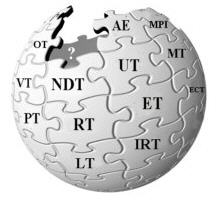
\includegraphics[scale=0.9]{img/ndtazWiki.jpg}
  \caption{NDT}
  \label{fig:ndtazWiki}
\end{figure}

\glqq Die Werkstoffprüfung umfasst verschiedene Prüfverfahren, mit denen das Verhalten und die
Werkstoffkenngrößen von normierten Werkstoffproben (Materialanalytik) oder fertigen Bauteilen
(Bauteilprüfung) unter mechanischen, thermischen oder chemischen Beanspruchungen ermittelt
werden.
Ein Werkstoff wird dabei hinsichtlich seiner Reinheit, Fehlerfreiheit oder Belastbarkeit überprüft. Nach
der Art werden die gängigen Prüfverfahren in zwei Hauptbereiche aufgeteilt: zerstörende und
zerstörungsfreie Werkstoffprüfung. Die auf die Abschätzung der Lebensdauer von Produkten und
Werkstoffen gerichteten Prüfungen fallen in das Gebiet der Umweltsimulation.\grqq
\footnote[1]{https://de.wikipedia.org/wiki/Werkstoffprüfung}
\\
VT: Vor jeder anderen zerstörungsfreien Prüfung wird eine Sichtprüfung durchgeführt. Dadurch
können erste Oberflächenfehler schnell und kostengünstig erkannt werden. Zur genaueren Analyse
ist meistens ein weiteres Prüfverfahren nötig.\\
\\
MT: Das Magnetpulverprüfverfahren dient dem Nachweis von Fehlern wie Rissen an der Oberfläche
oder im oberflächennahen Bereich von ferromagnetischen Werkstoffen. Durch das Verfahren wird
der, an einer fehlerhaften Stelle der Oberfläche, austretende magnetische Streufluss eines geeignet
magnetisierten Werkstücks sichtbar gemacht.\\
\\
\\
PT: Die (Farb-) Eindringprüfung ermöglicht mit einfachen Hilfsmitteln das Auffinden von Fehlern, die
bis zur Oberfläche hin offen sind. Das Verfahren kann bei jedem möglichen Material angewendet
werden.\\
\\
UT: Mit Hilfe der Ultraschallprüfung können flächige Fehler, wie Risse oder Bindefehler besonders
gut aufgefunden werden. Die Ultraschallprüfung wird üblicherweise im Impuls-Echoverfahren
durchgeführt.\\
\\
RT: Die Durchstrahlungsprüfung mittels Röntgen- oder Gammastrahlen eignet sich besonders zum
Auffinden von Volumenfehlern, wie Poren oder Lunker.\\
\\
\section{RT Durchstrahlungsprüfung}
\label{subsec:ndt}
Die Durchstrahlungsprüfung ist ein bildgebendes Verfahren der zerstörungsfreien Werkstoffprüfung (ZFP) zur Darstellung von Materialunterschieden.\\
Mit Röntgen- oder Gammastrahlung aus einer geeigneten Quelle (einer Röntgenröhre, einem Elektronenbeschleuniger mit Röntgentarget oder einem gammastrahlenden Radionuklid) wird die Dichte eines Bauteils auf einem Röntgenfilm abgebildet. Dort erscheint ein Projektionsbild des Bauteils. Am Grad der Schwärzung lässt sich die unterschiedliche Materialdicke oder -dichte erkennen. Je dicker oder dichter ein Bauteil, desto weniger Strahlung kann es durchdringen und desto heller erscheint die Stelle auf dem Röntgenbild.\\
\\
\subsection{Anwendung}
Die Röntgen- und Gammadurchstrahlung ist eine zerstörungsfreie Werkstoffprüfung zur Fehleraufdeckung im Inneren von Bauteilen, insbesondere an Schweißnähten von Blechen, Rohren und Behältern. Zur Prüfung sicherheitsrelevanter Bauteile bspw. von Schweißnähten (DIN EN ISO 10675-1) sowie sicherheitsrelevanter Gussteile (DIN EN 12681:2003-06 und DIN EN ISO 5579:2014-04) z. B. in Kraftwerken ist sie ein Standardverfahren.\\
Die häufigsten Fehler sind Lunker, Poren, Seigerungen und Risse. Damit diese gut erkennbar sind, müssen Strahlungsintensität, Wellenlänge der Strahlen, Dicke des Bauteils und Belichtungszeit aufeinander abgestimmt sein. Die Durchstrahlungsprüfung (Kürzel RT gem. DIN EN ISO 9712) ist geeignet zum Nachweis volumenhafter Fehler. Durch Unterschiede der Dichte zwischen Fehlstelle und Grundmaterial ist der Fehler nachweisbar. Auch feine Risse lassen sich bei geeignetem Einstrahlwinkel finden. Kontrast und Auflösung beeinflussen das Erkennen solcher Details. Der Kontrast ist abhängig von der Werkstoffdicke, der Dichte, dem Material, der Strahlerqualität/Energieintensität sowie dem Auflösungsvermögen und dem Typus des Films.\\
Zur Beurteilung der Bildgüte werden Karten (DIN EN ISO 19232-1:2013-12) mit sieben Drahtstegen unterschiedlicher Breite auf das belichtete Bauteil gelegt; die Drahtdurchmesser sind um 1,25 mm abgestuft. Anhand des dünnsten noch zu erkennenden Drahtes kann auf die kleinste erkennbare Fehlergröße geschlossen werden.\\
\\
\subsection{Eigenschaften}
Röntgen- und Gammastrahlen sind elektromagnetische Wellen. Physikalisch gleichen sie dem Licht, haben aber wesentlich kleinere Wellenlängen und dadurch höhere Frequenzen. Auf den kleinen Wellenlängen beruht die Fähigkeit, zwischen den Atomen der Materie einzudringen und mit genügend hoher Energie (Frequenz) auch durchzudringen (Bedingung: Wellenlänge muss kleiner als der Abstand zwischen den Atomen im Kristallgitter sein). Beim Durchdringen werden sie dann verschieden stark durch Fehler abgeschwächt und dadurch zeigt die austretende Strahlung Intensitätsunterschiede. Sie durchdringen Stahl bis etwa 300 mm, Leichtmetall bis 400 mm und Kupfer bis 50 mm. Das Durchdringungsvermögen der Röntgen- und Gammastrahlen ist umso höher, je kleiner die Dichte des Bauteils, die Wellenlänge der Strahlen und je größer die Frequenz ist. Gammastrahlen haben i. A. größere Eindringtiefen, weil sie kurzwelliger sind.\\
\\
\subsection{Erzeugung der Strahlen}
Gammastrahlen: Die wichtigsten Gammastrahler für die Werkstoffprüfung sind natürliche (Radium, Radon, Mesothor) und künstliche (Cobalt, Tantal, Cäsium, Thulium). Die Strahlenquelle ist ein zylinderförmiges und etwa 0,5 – 6 mm großes Präparat, das das jeweilige Radionuklid enthält. Da Gammastrahler nicht „ausgeschaltet“ werden können, sind sie gasdicht in der Strahlerkapsel mit Wolfram-Abschirmung (innen) und Blei- oder Uran-Abschirmung (außen) eingeschlossen, damit die Strahlung nicht allseitig austreten kann. Da die Strahlenquelle wesentlich kleiner als eine Röntgenröhre ist, lässt sie sich dichter an den Prüfling heranbringen, wie z. B. der Isotopenmolch, ein Gerät, das zur Schweißnahtprüfung auf Baustellen durch Rohre gezogen wird.
\\
\subsection{Nachweismöglichkeiten von Fehlern mit RT \ref{subsec:ndt}}

\subsubsection{Filmaufnahmen}
Die aus dem Werkstoff austretenden Strahlen treffen auf eine doppelbeschichtete Filmfolie, die auf der Rückseite mit Bleifolien abgedeckt ist, um Streustrahlen fernzuhalten. Intensitätsunterschiede setzen sich in Schwärzungsunterschiede des Films um. Durch unterschiedlich starke Schwärzungen des Films sieht man die geometrische Form sowie die Lage des Fehlers. Die Filmaufnahme ist mit Röntgen- und Gammastrahlen möglich.
Anwendung: Kontrolle von Schweißnähten und Gussteilen mit Dicken bis zu 100 mm (Stahl) und 400 mm (Al); Revisionsuntersuchungen in Kessel-, Brücken- und Flugzeugbau.\\
\subsubsection{Durchleuchtung mit Leuchtschirm}
Röntgenstrahlen regen bestimmte Kristalle zur Abgabe sichtbarer grün-gelber Strahlen an. Eine mit diesen Kristallen beschichtete Platte bildet den Leuchtschirm. Auf diesem erscheint ein Schattenbild des Prüflings, jedoch mit geringer Lichtstärke. Fehler mit geringer Dichte sind auf dem Schattenbild heller, Fehler mit höherer Dichte dunkler. Der Beobachter muss durch Bleiglas vor der Streustrahlung geschützt werden.
Anwendung: Die Durchleuchtung mit Röntgenstrahlen ist für Stahldicken bis zu 20 mm, für Leichtmetalle und Kunststoffe anwendbar.\\
\subsubsection{Röntgenbild-Verstärkerröhre}
Mit Hilfe von Elektronik kann das Röntgen-Leuchtschirmbild verkleinert und verstärkt werden. Das verstärkte (hellere) Bild kann fernsehtechnisch übertragen werden, so dass der Beobachter in einem strahlengeschützten Raum sitzen kann.
Anwendung: Prüfung von längs- und spiralgeschweißten Rohren.\\
\subsection{Art der durchdringenden Strahlung}
\begin{figure}[htb]
  \centering  
  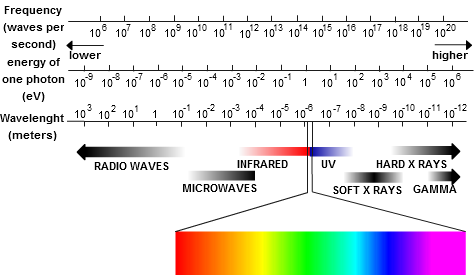
\includegraphics[scale=0.7]{img/ElectromagSpec.png}
  \caption{ElectromagSpec}
  \label{fig:ElectromagSpec}
\end{figure}
Onisierende Strahlung ist ein äußerst wichtiges Instrument der zerstörungsfreien Prüfung, es kann jedoch eine Gefahr für die menschliche Gesundheit darstellen. Aus diesem Grund sind besondere Vorsichtsmaßnahmen bei der Verwendung und dem Umgang mit ionisierender Strahlung zu beachten. Der Besitz radioaktiver Materialien und die Verwendung von Strahlung erzeugenden Geräten in den Vereinigten Staaten unterliegen strengen behördlichen Kontrollen. Die wichtigste Regulierungsbehörde für die meisten Arten und Verwendungen von radioaktiven Materialien ist die föderale Nuclear Regulatory Commission (NRC). Mehr als die Hälfte der Staaten in den USA haben jedoch eine "Vereinbarung" mit dem NRC getroffen, um die regulatorische Kontrolle der Verwendung radioaktiver Stoffe innerhalb ihrer Grenzen zu übernehmen. Im Rahmen des Einigungsprozesses müssen die Staaten Regelungen erlassen und durchsetzen, die mit denen in Titel 10 des Code of Federal Regulations vergleichbar sind. Vorschriften für die Kontrolle radioaktiven Materials in Iowa sind in Kapitel 136C des Iowa Code gefunden.
\footnote[2]{\url{https://www.nde-ed.org/index_flash.htm}}\\
In den meisten Fällen werden die Arten und die Höchstmengen an radioaktivem Material, die Art und Weise, in der sie verwendet werden dürfen, und die zur Verwendung radioaktiver Stoffe berechtigten Personen in Form einer "spezifischen" Genehmigung der zuständigen Aufsichtsbehörde festgelegt. In Iowa ist diese Behörde das Iowa Department of Public Health. Bei bestimmten Instituten, die routinemäßig große Mengen zahlreicher Arten radioaktiver Stoffe verwenden, sind die genauen Mengen an Materialien und Einzelheiten der Verwendung in der Lizenz möglicherweise nicht angegeben. Stattdessen räumt die Lizenz dem Organ die Befugnis und Verantwortung ein,die spezifischen Anforderungen für die Verwendung radioaktiver Stoffe in seinen Einrichtungen festzulegen.
Diese Lizenznehmer werden "Broadscope" genannt und erfordern ein Strahlensicherheits-Komitee und normalerweise einen Vollzeit-Strahlenschutzbeauftragten.\footnote[3]{\url{https://www.nde-ed.org/index_flash.htm}}\\

\subsection{Röntgenstrahlung}

\grqq Röntgenstrahlen sind wie jede andere Art von elektromagnetischer Strahlung. Sie können in Energiepaketen erzeugt werden, die Photonen genannt werden, genau wie Licht. Es gibt zwei verschiedene atomare Prozesse, die Röntgenphotonen erzeugen können. Einer wird Bremsstrahlung genannt und ist ein deutscher Begriff, der \grqq bremsende Strahlung\grqq bedeutet.\\Die andere wird K-Shell-Emission genannt. Sie können beide in den schweren Wolframatomen vorkommen. Wolfram ist oft das Material, das für das Target oder die Anode der Röntgenröhre gewählt wird.
Beide Arten, Röntgenstrahlen zu erzeugen, beinhalten eine Änderung des Zustands von Elektronen. Die Bremsstrahlung ist jedoch leichter zu verstehen, wenn man die klassische Idee verwendet, dass Strahlung emittiert wird, wenn sich die Geschwindigkeit des Elektronenstrahls auf das Wolfram ändert. Das negativ geladene Elektron verlangsamt sich nach dem Schwingen um den Kern eines positiv geladenen Wolframatoms. Dieser Energieverlust erzeugt Röntgenstrahlung. Elektronen werden durch den positiv geladenen Kern elastisch und inelastisch gestreut. Das inelastisch gestreute Elektron verliert Energie, die als Bremsstrahlung erscheint. Elastisch gestreute Elektronen (die rückgestreute Elektronen enthalten) werden im Allgemeinen durch größere Winkel gestreut. Bei der Wechselwirkung werden viele Photonen unterschiedlicher Wellenlängen erzeugt, aber keines der Photonen hat mehr Energie, als das Elektron hätte beginnen müssen. Nach dem Aussenden des Spektrums der Röntgenstrahlung wird das ursprüngliche Elektron abgebremst oder gestoppt.\grqq \\
\footnote[4]{\url{https://www.nde-ed.org/index_flash.htm}}\\
\begin{figure}[htb]
  \centering  
  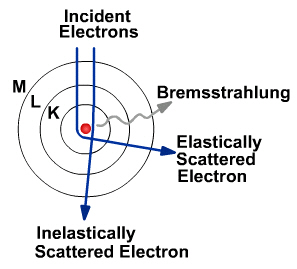
\includegraphics[scale=0.7]{img/Bremsstrahlung.jpg}
  \caption{Bremsstrahlung}
  \label{fig:Bremsstrahlung}
\end{figure}
\subsubsection{Bremsstrahlung}
Röntgenröhren erzeugen Röntgenphotonen, indem sie einen Elektronenstrom auf Energien von mehreren hundert Kilovolt mit Geschwindigkeiten von mehreren hundert Kilometern pro Stunde beschleunigen und zu einem schweren Targetmaterial kollidieren. Die abrupte Beschleunigung der geladenen Teilchen (Elektronen) erzeugt Bremsstrahlungsphotonen. Röntgenstrahlung mit einem kontinuierlichen Spektrum von Energien wird in einem Bereich von einigen keV bis zu einem Maximum der Energie des Elektronenstrahls erzeugt. Targetmaterialien für industrielle Röhren sind typischerweise Wolfram, was bedeutet, dass die Wellenfunktionen der gebundenen Wolframelektronen benötigt werden. Die inhärente Filtration einer Röntgenröhre muss berechnet werden, die durch die Menge kontrolliert wird, mit der das Elektron in die Oberfläche des Targets eindringt, und durch die Art des vorhandenen Vakuumfensters.\\
Die Bremsstrahlungsphotonen, die innerhalb des Targetmaterials erzeugt werden, werden abgeschwächt, wenn sie typischerweise 50 Mikrometer Targetmaterial passieren. Der Strahl wird durch das Aluminium- oder Beryllium-Vakuumfenster weiter gedämpft. Die Ergebnisse sind eine Eliminierung der Photonen mit niedriger Energie, 1 keV bis 15 keV, und eine signifikante Reduktion des Teils des Spektrums von 15 keV bis 50 keV. Das Spektrum von einer Röntgenröhre wird weiter durch die Filterung modifiziert, die durch die Auswahl von Filtern verursacht wird, die in dem Aufbau verwendet werden.
\subsection{Gammastrahlung}
Gammastrahlung ist eine der drei Arten natürlicher Radioaktivität. Gammastrahlen sind elektromagnetische Strahlung, wie Röntgenstrahlen. Die anderen beiden Arten natürlicher Radioaktivität sind Alpha- und Beta-Strahlung, die in Form von Teilchen vorliegen. Gammastrahlen sind die energiereichste Form elektromagnetischer Strahlung mit einer sehr kurzen Wellenlänge von weniger als einem Zehntel Nanometer.

Gammastrahlung ist das Produkt von radioaktiven Atomen. Abhängig vom Verhältnis von Neutronen zu Protonen in seinem Kern kann ein Isotop eines bestimmten Elements stabil oder instabil sein. Wenn die Bindungsenergie nicht stark genug ist, um den Kern eines Atoms zusammenzuhalten, wird das Atom als instabil bezeichnet. Atome mit instabilen Kernen verändern sich ständig infolge des Ungleichgewichts der Energie im Kern. Mit der Zeit zerfallen die Kerne von instabilen Isotopen spontan oder wandeln sich in einem Prozess, der als radioaktiver Zerfall bekannt ist. Verschiedene Arten von durchdringender Strahlung können von dem Kern und / oder seinen umgebenden Elektronen emittiert werden. Nuklide, die radioaktiv zerfallen, heißen Radionuklide. Jedes Material, das messbare Mengen eines oder mehrerer Radionuklide enthält, ist ein radioaktives Material.
Typen Strahlung, die durch radioaktives Zerfallsmaterial erzeugt wird.
Wenn ein Atom radioaktiv zerfällt, emittiert es eine oder mehrere Strahlungsformen mit ausreichender Energie, um die Atome zu ionisieren, mit denen es interagiert. Ionisierende Strahlung kann aus subatomaren Teilchen mit hoher Geschwindigkeit bestehen, die aus dem Kern ausgestoßen werden, oder aus elektromagnetischer Strahlung (Gammastrahlen), die entweder vom Kern oder den Orbitalelektronen emittiert wird.
\begin{figure}[htb]
  \centering  
  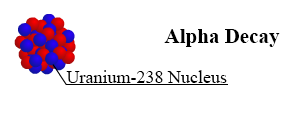
\includegraphics[scale=0.7]{img/uranium.png}
  \caption{Alpha-Zerfall}
  \label{fig:uranium}
Quelle: \url{https://www.nde-ed.org/index_flash.htm}
\end{figure}

 \subsubsection{Alpha-Strahlen}
 
\grqq Bestimmte Radionuklide mit hoher Atommasse (Ra226, U238, Pu239) zerfallen durch die Emission von Alphateilchen.Diese sind fest gebundene Einheiten von zwei Neutronen und zwei Protonen (He4-Kern) und haben eine positive Ladung. Die Emission eines Alphateilchens aus dem Kern führt zu einer Abnahme von zwei Einheiten der Ordnungszahl (Z) und vier Einheiten der Massenzahl (A). Alphateilchen werden mit diskreten Energien emittiert, die charakteristisch für die jeweilige Transformation sind, aus der sie stammen. Alle Alphateilchen aus einer bestimmten Radionuklidtransformation haben identische Energien.\grqq
\footnote[5]{\url{https://www.nde-ed.org/index_flash.htm}}\\
 \subsubsection{Beta-Strahlen}
\grqq Ein Kern mit einem instabilen Verhältnis von Neutronen zu Protonen kann durch die Emission eines Hochgeschwindigkeitselektrons, eines Betateilchens, zerfallen. Dies führt zu einer Nettoänderung von einer Einheit der Ordnungszahl (Z). Betateilchen haben eine negative Ladung, und die Betateilchen, die von einem spezifischen Radionuklid emittiert werden, liegen in einer Energie von nahe Null bis zu einem maximalen Wert, der für die bestimmte Transformation charakteristisch ist.\grqq
\footnote[6]{\url{https://www.nde-ed.org/index_flash.htm}}\\
 \subsubsection{Gamma-Strahlen}
 
\grqq Ein Kern, der sich in einem angeregten Zustand befindet, kann ein oder mehrere Photonen (Pakete elektromagnetischer Strahlung) diskreter Energien emittieren. Die Emission von Gammastrahlen verändert nicht die Anzahl von Protonen oder Neutronen im Kern, sondern bewirkt stattdessen, dass der Kern von einem höheren in einen niedrigeren Energiezustand (instabil bis stabil) bewegt wird. Die Gammastrahlenemission folgt häufig dem Beta-Zerfall, dem Alpha-Zerfall und anderen Kernzerfallsprozessen.\grqq
\footnote[7]{\url{https://www.nde-ed.org/index_flash.htm}}\\

\begin{figure}[htb]
  \centering  
  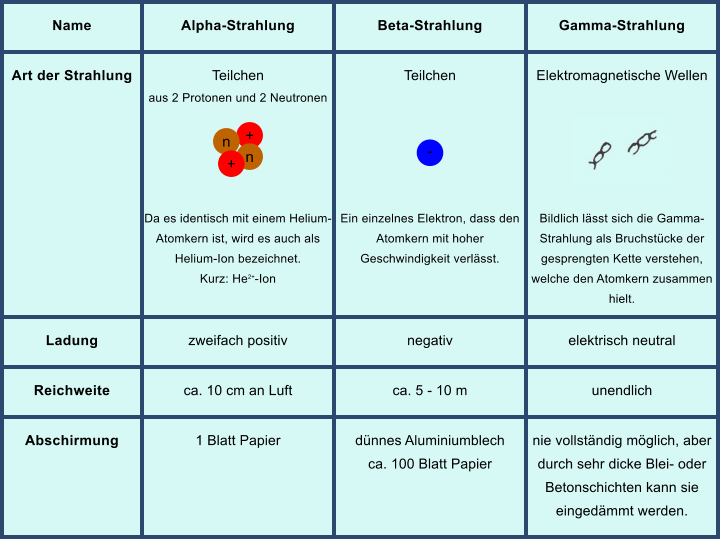
\includegraphics[scale=0.7]{img/strahlen.png}
  \caption{Die ionisierende Strahlung}
  \label{fig:strahlen}
  Quelle: \url{https://www.nde-ed.org/index_flash.htm}
\end{figure}
\subsection{Aktivität von Radionukliden}
Die Menge, die den Grad der Radioaktivität oder das Strahlungserzeugungspotential einer gegebenen Menge an radioaktivem Material ausdrückt, ist Aktivität.
Die Curie wurde ursprünglich als diejenige Menge von radioaktivem Material definiert, die mit der gleichen Geschwindigkeit wie ein Gramm reines Radium zerfällt.
Die Curie wurde seitdem genauer definiert als eine Menge radioaktiven Materials in
3.7 x 1010 Atome zerfallen pro Sekunde. Die Einheit des Internationalen Systems (SI) für die Aktivität ist das Becquerel (Bq), die Menge an radioaktivem Material, in der ein Atom pro Sekunde umgewandelt wird.
Die Radioaktivität einer gegebenen Menge an radioaktivem Material hängt nicht von der Masse des vorhandenen Materials ab.
Zum Beispiel könnten zwei Ein-Curie-Quellen von Cs-137 sehr unterschiedliche Massen haben, abhängig von dem relativen Anteil von nicht-radioaktiven Atomen, die in jeder Quelle vorhanden sind. Die Radioaktivität wird als die Anzahl von Curie oder Becquerel pro Massen- oder Volumeneinheit ausgedrückt.
\begin{figure}[htb]
  \centering  
  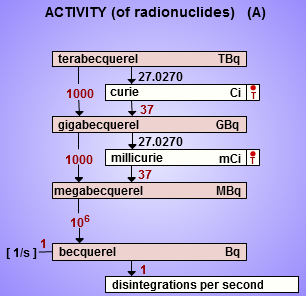
\includegraphics[scale=0.8]{img/activity.png}
  \caption{Radioaktivität}
  \label{fig:activity}
   Quelle: \url{https://www.nde-ed.org/index_flash.htm}
\end{figure}
Die Konzentration der Radioaktivität oder die Beziehung zwischen der Masse des radioaktiven Materials und der Aktivität wird "spezifische Aktivität" genannt. Die spezifische Aktivität wird ausgedrückt als die Anzahl der Curie oder Becquerel pro Massen- oder Volumeneinheit. Jedes Gramm Cobalt-60 enthält etwa 50 Curies. Iridium-192 enthält 350 Curies für jedes Gramm Material.
Je kürzer die Halbwertszeit, desto weniger Material wird benötigt, um eine bestimmte Aktivität zu erzeugen oder zu curieren.
Die höhere spezifische Aktivität von Iridium führt zu physikalisch kleineren Quellen. Dies ermöglicht es den Technikern, die Quelle näher an den Film zu legen, während die geometrischen Unschärfeanforderungen auf dem Röntgenbild beibehalten werden.
Diese Unschärfebedingungen können möglicherweise nicht erfüllt werden, wenn eine Quelle mit einer geringen spezifischen Aktivität bei ähnlichen Abständen von Quelle zu Film verwendet wird.
\subsection{Isotopenabfallrate (Halbwertszeit)}
Jedes Radionuklid zerfällt mit seiner eigenen einzigartigen Geschwindigkeit, die durch keine chemischen oder physikalischen Prozesse verändert werden kann. Ein nützliches Maß für diese Geschwindigkeit ist die Halbwertszeit des Radionuklids. Die Halbwertszeit ist definiert als die Zeit, die erforderlich ist, damit die Aktivität eines bestimmten Radionuklids auf die Hälfte seines Anfangswertes absinkt. Mit anderen Worten, die Hälfte der Atome ist zu einem stabileren Zustand zurückgekehrt. Die Halbwertszeiten von Radionukliden reichen von Mikrosekunden bis Milliarden von Jahren. Die Halbwertszeit von zwei weit verbreiteten industriellen Isotopen beträgt 74 Tage für Iridium-192 und 5,3 Jahre für Kobalt-60. Genauere Berechnungen können für die Halbwertszeit dieser Materialien gemacht werden, jedoch werden diese Zeiten üblicherweise verwendet.
\begin{figure}[htb]
  \centering  
  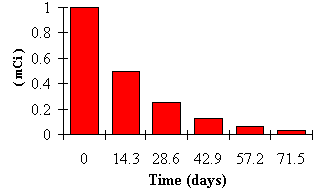
\includegraphics[scale=0.5]{img/halbwertszeit.png}
  \caption{Isotopen Halbwertszeit}
  \label{fig:halbwertszeit}
   Quelle: \url{https://www.nde-ed.org/index_flash.htm}
\end{figure}

Das Applet bietet eine interaktive Darstellung der radioaktiven Zerfallsreihen.
Die vier dargestellten Serien sind Th232, Ir192, Co60, Ga75 und C14.

\subsection{Halbwertsschicht}
Die Dicke eines gegebenen Materials, bei dem 50\% der einfallenden Energie gedämpft wurden, ist als Halbwertschicht (HVL) bekannt. Die HVL wird in Entfernungseinheiten (mm oder cm) ausgedrückt. Wie der Dämpfungskoeffizient ist es abhängig von der Photonenenergie. Die Erhöhung der Durchdringungsenergie eines Photonenstroms führt zu einer Erhöhung der HVL eines Materials.

Die HVL ist umgekehrt proportional zum Dämpfungskoeffizienten. Wenn eine einfallende Energie von 1 und eine übertragene Energie von 0,5 in die auf der vorhergehenden Seite eingeführte Gleichung eingesteckt wird, kann man sehen, dass die HVL mit m multipliziert wird.
 \begin{figure}[htb]
 \centering 
  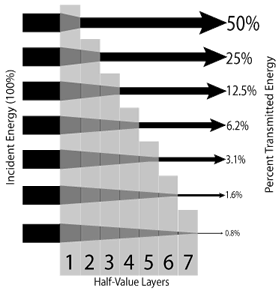
\includegraphics[scale=0.9]{img/Half-Value-Layer.png}
  \caption{Half-Value-Layer}
  \label{fig:Half-Value-Layer}
   Quelle: \url{https://www.nde-ed.org/index_flash.htm}
  \end{figure}


Wenn x die HVL ist, dann muss m HVL gleich 0,693 sein (da die Zahl 0,693 der Exponentenwert ist, der einen Wert von 0,5 ergibt).

\begin{figure}[htb]
  \centering  
  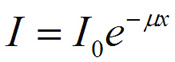
\includegraphics[scale=0.5]{img/Die_Kurve_Formel.jpg}
\end{figure}

\begin{figure}[htb]
  \centering  
  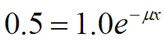
\includegraphics[scale=0.5]{img/IntensityEq5.jpg}
  \caption{IntensityEq5}
  \label{fig:IntensityEq5}
   Quelle: \url{https://www.nde-ed.org/index_flash.htm}
\end{figure}

  \subsubsection{Half-Value-Layer}
Die HVL wird häufig in der Radiographie verwendet, weil es einfacher ist, sich Werte zu merken und einfache Berechnungen durchzuführen. Bei einer Abschirmungsberechnung, wie sie rechts dargestellt ist, kann gesehen werden, dass, wenn die Dicke einer HVL bekannt ist, schnell bestimmt werden kann, wie viel Material benötigt wird, um die Intensität auf weniger als 1\% zu reduzieren.\\
\\
Daher sind die HVL und m wie folgt verwandt:
\begin{figure}[htb]
\centering 
  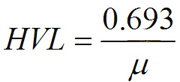
\includegraphics[scale=0.5]{img/IntensityEq6.jpg}
  \caption{IntensityEq6}
  \label{fig:IntensityEq6}
  
  \end{figure}
  \subsubsection{Approximate HVL für verschiedene Materialien mit Gamma Quelle}
  {\rowcolors{3}{yellow}{green}
\begin{tabular}{ |p{3cm}||p{2cm}|p{2cm}|p{2cm}|p{2cm}|p{2cm}| }
 \hline
 \multicolumn{6}{|c|}{ Half-Value Layer, mm (inch)} \\
 \hline
 Source& Concrete &Steel &Lead&Tungsten&Uranium\\
  \hline
 Iridium-192 & 44.5 (1.75)&12.7 (0.5)&4.8 (0.19)&3.3 (0.13)&2.8 (0.11)\\
  \hline
 Cobalt-60   &60.5 (2.38)&21.6 (0.85)&12.5 (0.49)&7.9 (0.31)&6.9 (0.27)\\
 \hline
\end{tabular} 
\subsubsection{Approximate HVL für verschiedene Materialien mit X-ray Quelle}

{\rowcolors{3}{yellow}{green}

\begin{tabular}{ |p{4cm}||p{3cm}|p{3cm}|  }
\hline
\multicolumn{3}{|c|}{Half-Value Layer, mm (inch)} \\
\hline
Peak Voltage (kVp) & Lead&Concrete \\
\hline
50&0.06 (0.002)& 4.32 (0.170) \\
\hline
100	&0.27 (0.010)&15.10 (0.595) \\
\hline
150	&0.30 (0.012)& 22.32 (0.879) \\
\hline
200& 0.52 (0.021) & 25.0 (0.984) \\
\hline
250& 0.88 (0.035)&28.0 (1.102)  \\
\hline
300& 1.47 (0.055) & 31.21 (1.229) \\
\hline
400& 2.5 (0.098)& 33.0 (1.299) \\
\hline
1000&7.9 (0.311) & 44.45 (1.75)\\
\hline
\end{tabular} \\


\subsection{Ionisation}
Da sich die durchdringende Strahlung in Materie von Punkt zu Punkt bewegt, verliert sie ihre Energie durch verschiedene Wechselwirkungen mit den Atomen, auf die sie trifft.
Die Geschwindigkeit, mit der dieser Energieverlust abhängt, durch welche von der Art und Energie der Strahlung und der Dichte und der atomaren Zusammensetzung der Materie tritt es passiert.
Die verschiedenen Arten von durchdringender Strahlung übertragen ihre Energie hauptsächlich durch Anregung und Ionisation von Orbitalelektronen. Der Begriff „Anregung“ wird verwendet, um eine Wechselwirkung zu beschreiben, wo Elektronen Energie von einem vorbeifahrenden geladenen Teilchen zu erwerben, sind jedoch nicht vollständig von ihrem Atom entfernt. Aufgeregte Elektronen können anschließend Energie in Form von Röntgenstrahlen während des Prozesses der Rückkehr in einen niedrigeren Energiezustand emittieren. Der Begriff "Ionisierung" bezieht sich auf die vollständige Entfernung eines Elektrons von einem Atom nach der Übertragung von Energie von einem passierenden geladenen Teilchen. Bei der Beschreibung der Intensität der Ionisation wird häufig der Begriff "spezifische Ionisation" verwendet. Dies ist definiert als die Anzahl von Ionenpaaren, die pro Weglängeneinheit für eine gegebene Art von Strahlung gebildet werden.

\begin{figure}[htb]
  \centering  
  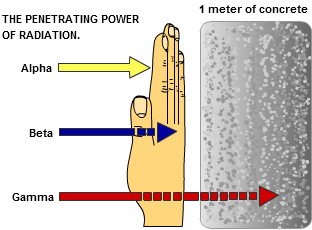
\includegraphics[scale=0.5]{img/Ionisation.png}
  \caption{Ionisation}
  \label{fig:Ionisation}
  Quelle: \url{https://www.nde-ed.org/index_flash.htm}
\end{figure}

Aufgrund ihrer doppelten Ladung und relativ langsamen Geschwindigkeit haben Alphateilchen eine hohe spezifische Ionisierung und eine relativ kurze Reichweite in der Materie (einige Zentimeter in Luft und nur Bruchteile von einem Millimeter im Gewebe). Betateilchen haben eine viel geringere spezifische Ionisierung als Alphateilchen und im allgemeinen einen größeren Bereich. Zum Beispiel haben die relativ energiereichen Betateilchen von P32 eine maximale Reichweite von sieben Metern in der Luft und acht Millimeter im Gewebe. Die niederenergetischen Betas von H3 werden andererseits nur von sechs Millimetern Luft oder sechs Mikrometern Gewebe gestoppt.
Gammastrahlen, Röntgenstrahlen und Neutronen werden als indirekt ionisierende Strahlung bezeichnet, da sie, ohne Ladung, nicht direkt Impulse an die Orbitalelektronen abgeben, wie es Alpha- und Betateilchen tun. Elektromagnetische Strahlung durchläuft Materie, bis eine Wechselwirkung mit einem Teilchen möglich ist. Wenn das Teilchen ein Elektron ist, kann es genug Energie erhalten, um ionisiert zu werden, woraufhin es eine weitere Ionisierung durch direkte Wechselwirkungen mit anderen Elektronen bewirkt. Als Ergebnis kann indirekt ionisierende Strahlung (z. B. Gamma, Röntgenstrahlen und Neutronen) die Freisetzung von direkt ionisierenden Teilchen (Elektronen) tief in einem Medium verursachen. Da diese neutralen Strahlungen nur zufällige Begegnungen mit Materie erfahren, haben sie keine endlichen Bereiche, sondern werden exponentiell abgeschwächt. Mit anderen Worten, ein gegebener Gammastrahl hat eine bestimmte Wahrscheinlichkeit, irgendein Medium irgendeiner Tiefe zu durchqueren.\\
Neutronen verlieren Energie in Materie durch Kollisionen, die kinetische Energie übertragen. Dieser Vorgang wird Moderation genannt und ist am effektivsten, wenn die Materie, mit der die Neutronen kollidieren, etwa die gleiche Masse wie das Neutron hat. Wenn die Neutronen einmal auf die gleiche durchschnittliche Energie abgebremst sind wie die Materie, mit der sie interagiert (thermische Energien), haben sie eine viel größere Chance, mit einem Kern in Wechselwirkung zu treten. Solche Wechselwirkungen können dazu führen, dass Material radioaktiv wird oder Strahlung abgeben kann.

\subsection{Newtons umgekehrtes quadratisches Gesetz für die Intensität}

Jede Punktquelle, die ihren Einfluss gleichmäßig in alle Richtungen ausbreitet, ohne eine Begrenzung ihrer Reichweite zu haben, wird dem Gesetz des umgekehrten Quadrats folgen. Dies ergibt sich aus streng geometrischen Überlegungen. Die Intensität des Einflusses bei jedem gegebenen Radius (r) ist die Quellenstärke dividiert durch die Fläche der Kugel. Das Gesetz des umgekehrten Quadrats, das streng geometrisch ist, gilt für verschiedene Phänomene. Punktquellen der Gravitationskraft, des elektrischen Feldes, des Lichts, des Schalls und der Strahlung folgen dem umgekehrten Quadratgesetz.
Als eines der Felder, die dem allgemeinen inversen Quadratgesetz folgen, kann eine Punktstrahlungsquelle durch das obige Diagramm charakterisiert werden, ob Sie von Röntgen, Rad oder Rem sprechen. Alle Belichtungsmaße werden durch das umgekehrte Quadratgesetz fallen.
Wenn zum Beispiel die Strahlenbelastung 100 mR / h bei 1 Inch von einer Quelle beträgt, beträgt die Belichtung 0,01 mR / h bei 100 Inch.
Das Applet unten zeigt eine radioaktive Quelle. Die Entfernung zur grünen Quelle wird unten angezeigt.
\begin{figure}[htb]
  \centering  
  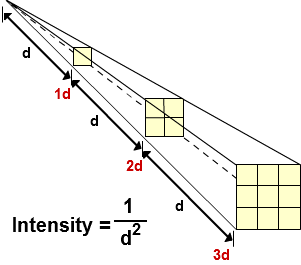
\includegraphics[scale=0.7]{img/Intensitaet.png}
  \caption{Intensität}
  \label{fig:Intensität}
  Quelle: \url{https://www.nde-ed.org/index_flash.htm}
\end{figure}

\subsection{Wechselwirkung zwischen eindringender Strahlung
und Materie}
Wenn Röntgenstrahlen oder Gammastrahlen in ein Objekt gerichtet werden, interagieren einige der Photonen mit den Teilchen der Materie und ihre Energie kann absorbiert oder gestreut werden. Diese Absorption und Streuung wird als Dämpfung bezeichnet. Andere Photonen wandern vollständig durch das Objekt, ohne mit einem der Teilchen des Materials in Wechselwirkung zu treten. Die Anzahl der Photonen, die durch ein Material durchgelassen werden, hängt von der Dicke, Dichte und Atomzahl des Materials und der Energie der einzelnen Photonen ab.
\begin{figure}[htb]
  \centering  
  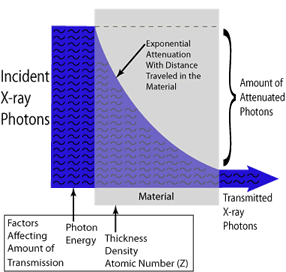
\includegraphics[scale=0.6]{img/wechselwirkungstrahlung1.png}
  \caption{wechselwirkungstrahlung1}
  Quelle: \url{https://www.nde-ed.org/index_flash.htm}
  \label{fig:strahlung1}
\end{figure}
Selbst wenn sie die gleiche Energie haben, bewegen sich Photonen in einem Material in unterschiedlichen Abständen, einfach aufgrund der Wahrscheinlichkeit ihrer Begegnung mit einem oder mehreren Teilchen der Materie und der Art der Begegnung.
Da die Wahrscheinlichkeit einer Begegnung mit der zurückgelegten Entfernung zunimmt, nimmt die Anzahl der Photonen, die einen bestimmten Punkt innerhalb der Materie erreichen, exponentiell mit der zurückgelegten Entfernung ab.
Wie in der Grafik gezeigt, wenn 1000 Photonen auf zehn 1 cm-Schichten eines Materials gerichtet sind und eine 10\% Wahrscheinlichkeit besteht, dass ein Photon in dieser Schicht gedämpft wird, werden 100 Photonen abgeschwächt. Dies lässt 900 Fotos in die nächste Schicht,in denen 10\% dieser Fotos abgeschwächt werden.
Durch Fortsetzen dieses Verlaufs wird die exponentielle Form der Kurve offensichtlich.
\begin{figure}[htb]
  \centering  
  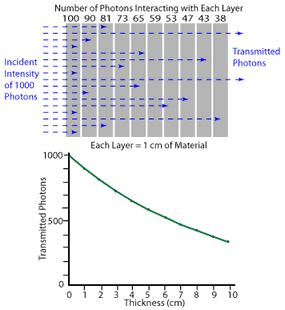
\includegraphics[scale=0.7]{img/wechselwirkungstrahlung2.png}
  \caption{wechselwirkungstrahlung2}
  \label{fig:strahlung2}
  Quelle: \url{https://www.nde-ed.org/index_flash.htm}
\end{figure}

















 
 
 




\chapter{Stand der Technik}
\label{cha:stand_der_technik}

\section{RT Technik}

\subsection{Geometrische Unschärfe }
\label{sec:ndt}

Geometrische Unschärfe bezieht sich auf den Verlust der Definition, der das Ergebnis geometrischer Faktoren der radiographischen Ausrüstung und des Aufbaus ist.Es tritt auf, weil die Strahlung nicht von einem einzelnen Punkt, sondern über eine Fläche stammt.
Betrachten Sie die Bilder unten, die zwei Quellen unterschiedlicher Größe zeigen, die Strahlengänge von jeder Kante der Quelle zu jeder Kante des Merkmals der Probe, die Stellen, an denen diese Strahlung den Film belichtet, und das Dichteprofil über den Film. Im ersten Bild stammt die Strahlung von einer sehr kleinen Quelle. Da die gesamte Strahlung im wesentlichen aus dem gleichen Punkt stammt, wird im Bild sehr wenig geometrische Unschärfe erzeugt. In dem zweiten Bild ist die Quellengröße größer und die verschiedenen Wege, die die Strahlungsstrahlen von ihrem Ursprungspunkt in der Quelle nehmen können, bewirken, dass die Kanten der Einkerbung weniger definiert sind.\\
\subsubsection{GeometricUnsharpness}
\begin{figure}[htb]
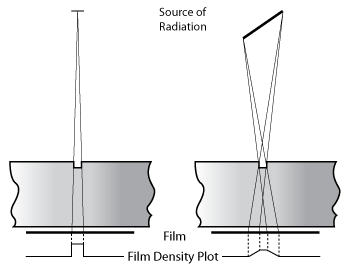
\includegraphics[scale=0.5]{img/GeometricUnsharpness.png}\\
\label{sec:GeometricUnsharpness}
  \caption{GeometricUnsharpness}
  \label{sec:geometricUnsharpness1}
  \end{figure}

Die drei Faktoren, die die Unschärfe steuern, sind die Quellengröße, die Entfernung von Quelle zu Objekt und die Distanz zwischen Objekt und Detektor. Die Quellengröße wird durch Bezugnahme auf Herstellerspezifikationen für eine gegebene Röntgen- oder Gammastrahlenquelle erhalten. Industrieröntgenröhren haben häufig Brennfleckgrößen von 1,5 mm im Quadrat, Mikrofokussysteme haben jedoch Fleckgrößen im Bereich von 30 Mikron. Wenn die Quellengröße abnimmt, nimmt auch die geometrische Unschärfe ab. Für eine Quelle mit gegebener Größe kann die Unschärfe ebenfalls durch Erhöhen der Entfernung von der Quelle zum Objekt verringert werden, dies führt jedoch zu einer Verringerung der Strahlungsintensität.
Der Abstand zwischen Objekt und Detektor wird normalerweise so klein wie möglich gehalten, um die Unschärfe zu minimieren. Es gibt jedoch Situationen, z. B. bei Verwendung einer geometrischen Vergrößerung, wenn das Objekt vom Detektor getrennt wird, was die Definition verringert. Das unten stehende Applet ermöglicht die Visualisierung der geometrischen Unschärfe, wenn Quellgröße, Entfernung von Quelle zu Objekt und Abstand zwischen Quelle und Detektor variiert werden. Der Bereich mit unterschiedlicher Dichte am Rand eines Features, der sich aufgrund geometrischer Faktoren ergibt, wird als Penumbra bezeichnet.

Codes und Standards, die in der industriellen Radiographie verwendet werden, erfordern, dass geometrische Unschärfe begrenzt wird. Im Allgemeinen beträgt die zulässige Menge 1/100 der Materialdicke bis zu einem Maximum von 0,040 Zoll. Diese Werte beziehen sich auf den Grad des Halbschattens in einem Röntgenbild.
Da die Penumbra nicht annähernd so gut definiert ist, wie in der Abbildung(\ref{sec:geometricUnsharpness})gezeigt, ist es schwierig, sie in einem Röntgenbild zu messen. Daher wird es typischerweise berechnet.
Die Quellengröße muss vom Gerätehersteller bezogen oder gemessen werden. Dann kann die Unschärfe anhand von Messungen des Setups berechnet werden.
Für den Fall, wie rechts gezeigt, wo eine Probe mit einer signifikanten Dicke in der Nähe des Detektors platziert wird, wird die folgende Formel verwendet, um die maximale Menge an Unschärfe aufgrund der Probendicke zu berechnen:\\

  Ug = f * b/a

f = Quelle Brennpunktsgröße (source focal-spot size) \\
a = Abstand von der Quelle zur vorderen Oberfläche des Objekts\\
b = Die Dicke des Objekts\\
\begin{figure}[htb]
  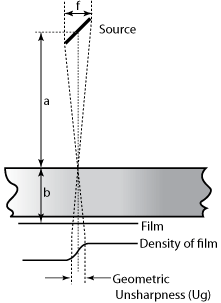
\includegraphics[scale=0.9]{img/GeometricUnsharpness2.png}\\
  \caption{GeometricUnsharpness2}
  \label{sec:geometricUnsharpness}
  \end{figure}
Für den Fall, dass der Detektor nicht neben der Probe platziert wird, etwa wenn eine geometrische Vergrößerung verwendet wird, wird die Berechnung zu:\\

Ug = f* b/a\\
f = Quelle Brennpunktsgröße (source focal-spot size) \\
a = Abstand von der Röntgenquelle(x-ray) zur vorderen Oberfläche des Materials / Objekts\\
b = Die Dicke des Objekts\\
\begin{figure}[htb]
  \centering 
 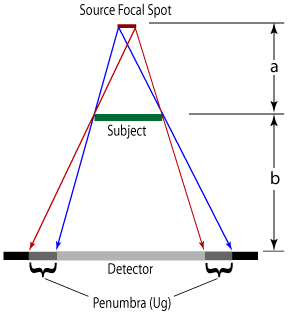
\includegraphics[scale=0.9]{img/Penumbra.png}
 \caption{Penumbra}
  \label{fig:Penumbra}
\end{figure}

\label{sec:RT Technik}
\section{Sekundäre Strahlung und Unterschnittkontrolle}
\label{sec:Strahlung und Unterschnittkontrolle}
Quelle: \url{https://www.nde-ed.org/index_flash.htm}
\subsection{Sekundäre Strahlung}
Sekundär- oder Streustrahlung muss oft bei der Erstellung eines Röntgenbildes berücksichtigt werden. Die gestreuten Photonen erzeugen einen Verlust von Kontrast und Definition. Häufig wird Sekundärstrahlung als Strahlung angesehen, die auf den Film trifft, der von einem Objekt in der unmittelbaren Umgebung, wie einer Wand, oder von dem Tisch oder Boden, auf dem das Teil ruht, reflektiert wird. Seitliche Streuung entsteht von Wänden oder Objekten auf der Quellseite des Films. Die Steuerung der Seitenstreuung kann erreicht werden, indem Objekte in dem Raum weg von dem Film bewegt werden, die Röntgenröhre in die Mitte des Gewölbes bewegt wird oder ein Kollimator an der Austrittsöffnung platziert wird, wodurch die divergierende Strahlung um den Zentralstrahl reduziert wird.
\begin{figure}[htb]
 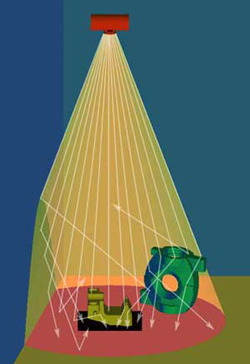
\includegraphics[scale=0.7]{img/XRSIM-Scatter2aS.jpg}
 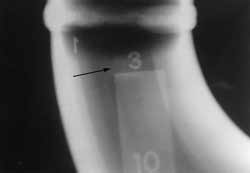
\includegraphics[scale=0.9]{img/BackScatter(small).jpg}
 \caption{BackScatter}
 Quelle: \url{https://www.nde-ed.org/index_flash.htm}
  \label{fig:BackScatter}
\end{figure}
Es wird oft als Rückstreuung bezeichnet, wenn es von Objekten hinter dem Film kommt. Industriestandards und Standards verlangen oft, dass ein Buchstabe B auf der Rückseite der Kassette platziert wird, um die Kontrolle der Rückstreuung zu überprüfen.

Wenn der Buchstabe B als ein Geister -Bild auf dem Film erscheint, erreicht eine signifikante Menge an Rückstreustrahlung den Film. Das Bild des B ist oft sehr unscharf,
(BILD \ref{fig:BackScatter}). Der Pfeil zeigt auf das Gebiet der Rückstreustrahlung von der Leitung B, die sich auf der Rückseite des Films befindet. Die Steuerung der Rückstreustrahlung wird erreicht, indem der Film in der Kassette mit einer mindestens 0,010 Zoll dicken Bleifolie hinterlegt wird. Es ist eine übliche Praxis in der Industrie, einen 0,005-Zoll-Führungsschirm vor und einen 0,010-Zoll-Schirm hinter dem Film anzuordnen.
\subsection{Unterschnitt}
Eine weitere Bedingung, die oft bei der Erstellung eines Röntgenbildes kontrolliert werden muss, ist Undercut. Teile mit Löchern, hohlen Bereichen oder abrupten Dickenänderungen werden wahrscheinlich durch Unterschnitte beeinträchtigt, wenn die Bedienelemente nicht eingesetzt werden. Hinterschnitt erscheint als Verdunkelung des Röntgenbildes im Bereich des Dickenübergangs. Dies führt zu einem Verlust der Auflösung oder Unschärfe im Übergangsbereich. Unterschneidung tritt aufgrund von Streuung innerhalb des Films auf.\\

An den Rändern eines Teils oder der Bereiche, wo der Teil von dick zu dünn übergeht, ist die Intensität der Strahlung, die den Film erreicht, viel größer als in den dickeren Bereichen des Teils. Die hohe Strahlungsintensität, die den Film erreicht, führt zu einer hohen Streuung innerhalb des Films. Es sollte auch beachtet werden, dass, je schneller die Filmgeschwindigkeit ist, desto mehr Unterschneidung wahrscheinlich auftritt. Streuung innerhalb der Wände des Teils trägt ebenfalls zur Unterschneidung bei, aber die Forschung hat gezeigt, dass die Streuung innerhalb des Films die Hauptursache ist. Masken dienen zur Kontrolle der Unterschneidung. Als Masken werden häufig Bleibleche verwendet, die zum Füllen von Löchern oder zum Umschließen des Teils geschnitten werden, und metallische Schrot- und Flüssigkeitsabsorber.

\begin{figure}[htb]
  \centering 
 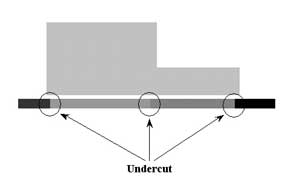
\includegraphics[scale=0.9]{img/Undercut.jpg}
 \caption{Undercut}
  \label{fig:Undercut}
  Quelle: \url{https://www.nde-ed.org/index_flash.htm}
\end{figure}
\begin{figure}[h]
 %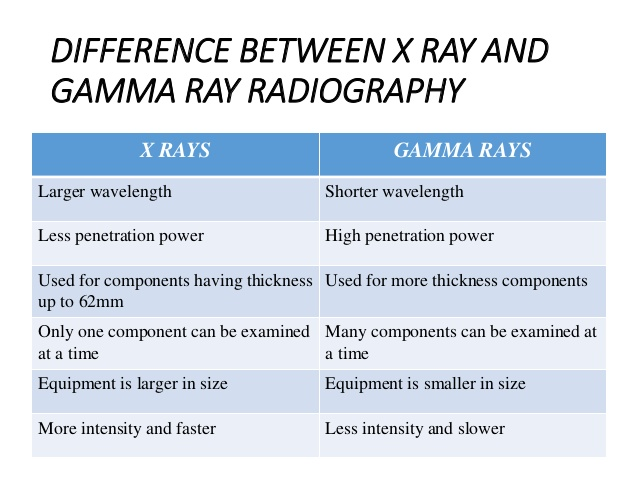
\includegraphics[scale=0.5]{img/gammaAndx-ray.jpg}
   \centering
 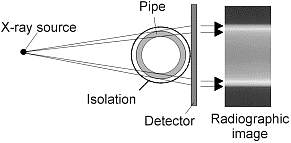
\includegraphics[scale=0.5]{img/x-ray.png}
 \caption{X-Ray}
  \label{fig:gammaAndx-ray}
  \centering
  Quelle: \url{https://www.nde-ed.org/index_flash.htm}
\end{figure}

\section{Filter in der Radiographie}
\subsection{X-Ray}

Bei Röntgenenergien bestehen Filter aus Material, das in dem Nutzstrahl angeordnet ist, um vorzugsweise Strahlung basierend auf dem Energieniveau zu absorbieren oder die räumliche Verteilung des Strahls zu modifizieren. Die Filtration wird benötigt, um die Röntgenstrahlen mit niedrigerer Energie zu absorbieren, die von der Röhre emittiert werden, bevor sie das Ziel erreichen. Die Verwendung von Filtern erzeugt ein saubereres Bild durch Absorbieren der Röntgenstrahlenphotonen mit niedrigerer Energie, die dazu neigen, mehr zu streuen.

Die Gesamtfiltration des Strahls umfasst die inhärente Filtration (bestehend aus einem Teil der Röntgenröhre und des Röhrengehäuses) und die hinzugefügte Filterung (dünne Bleche eines Metalls, das in den Röntgenstrahl eingeführt wird). Filter werden typischerweise in der Nähe des Röntgenstrahlkanals im direkten Weg des Röntgenstrahls angeordnet. Auch eine dünne Kupferfolie zwischen dem Teil und der Filmkassette hat sich als eine effektive Filtrationsmethode erwiesen.

Für die industrielle Radiographie werden die Filter, die dem Röntgenstrahl hinzugefügt werden, meistens aus Materialien mit hoher Kernladungszahl wie Blei, Kupfer oder Messing hergestellt. Filter für die medizinische Radiographie bestehen in der Regel aus Aluminium (Al). Die Menge sowohl der inhärenten als auch der zugesetzten Filtration wird in mm Al oder mm Al-Äquivalent angegeben. Die Filtrationsmenge des Röntgenstrahls wird spezifiziert durch und basiert auf dem Spannungspotential (keV), das verwendet wird, um den Strahl zu erzeugen. Die Dicke der Filtermaterialien hängt von Ordnungszahlen, Kilovolt-Einstellungen und dem gewünschten Filtrationsfaktor ab.

\subsection{Gamma}
Gammaradiographie erzeugt relativ hohe Energieniveaus bei im wesentlichen monochromatischer Strahlung, daher ist die Filtration keine nützliche Technik und wird selten verwendet.\\



\subsection{RT-Ressourcen}
\label{sec:resourcen}
\begin{enumerate}
\item Personal: mindestens 2
\begin{itemize}
\item Health Physics Safety(HPS)
\item Radiographer
\item Assistance
\end{itemize}
\item Haupt-Materialien 
\begin{itemize}
\item Materialien
\begin{itemize}
\item Radioaktive Isotope z.B. Iridium-192
\item Gamma Radiation Projection Devices z.B.
\href{https://www.ndt.com.au/product/qsa-sentinel-iridium-ir-192-sources-for-gamma-radiography/}{\textcolor{blue}{SENTINEL}}
\item Film z.B.
\href{https://www.gemeasurement.com/sites/gemc.dev/files/geit-40007-structurix_en_04-17.pdf}{\textcolor{blue}{AGFA}} 
\end{itemize}
\item Prozess-Materialien
\begin{itemize}
\item Chemikalien für Filmentwickler und Filmfixierer z.B. \href{https://www.gemeasurement.com/sites/gemc.dev/files/geit-40007-structurix_en_04-17.pdf}{\textcolor{blue}{AGFA}}
\item Dunkelkammer für Entwicklung z.B.
\href{https://www.gemeasurement.com/sites/gemc.dev/files/structurix_processing_equipment_brochure_english.pdf}{\textcolor{blue}{Digitale Dunkelkammer}}
\end{itemize}
\item Sicherheit-Materialien
\begin{itemize}
\item Personal Dosimetrie z.B.\\
\href{https://www.pce-instruments.com/deutsch/messtechnik/messgeraete-fuer-alle-parameter/geigerzaehler-kat_10582_1.htm}{\textcolor{blue}{Geiger-Müller-Alarm},}\\
\href{https://de.wikipedia.org/wiki/Thermolumineszenzdosimeter}{\textcolor{blue}{Thermolumineszenzdosimeter (TLD)},}\\
\href{https://en.wikipedia.org/wiki/Film_badge_dosimeter}{\textcolor{blue}{Film badge dosimeter},\\ \textcolor{blue}{...}}
\item Strahlungsbereich Dosimetrie z.B.
\href{https://www.gamma-scout.com/DE/Technische-Daten.php}{\textcolor{blue}{GAMMA-SCOUT-Radiometer}}
\item Strahlungszeichen z.B. 
\href{https://de.wikipedia.org/wiki/Strahlenwarnzeichen}{\textcolor{blue}{Zeichen für Strahlungsbereich}}
\item Strahlenbelastung-Notfall z.B. 
\href{http://www.gilligan-engineering.co.uk/news/71-emergency-source-containers}{\textcolor{blue}{Notfall-Aufbewahrungsbehälter}} 
\end{itemize}
\end{itemize}
\end{enumerate}















\chapter{Sicherheit}
\label{chap:Sicherheit}

\section{Halbwertschicht (Abschirmung)}
\label{sec:Halbwertschicht }
Wie im vor Abschnitt über die Strahlungstheorie diskutiert wurde, hängt die Eindringtiefe für eine gegebene Photonenenergie von der Materialdichte (Atomstruktur) ab. Je mehr subatomare Teilchen in einem Material vorliegen (höhere Z-Zahl), desto größer ist die Wahrscheinlichkeit, dass Wechselwirkungen auftreten und die Strahlung ihre Energie verliert. Je dichter ein Material ist, desto geringer ist daher die Eindringtiefe der Strahlung. Materialien wie abgereichertes Uran, Wolfram und Blei haben hohe Z-Zahlen und sind daher sehr wirksam bei der Abschirmung von Strahlung. Beton ist nicht so wirksam in der Abschirmung von Strahlung, aber es ist ein sehr gebräuchliches Baumaterial und wird daher häufig bei der Konstruktion von Strahlungsgewölben verwendet.\\
Da unterschiedliche Materialien die Strahlung in unterschiedlichem Maße abschwächen, wurde ein praktisches Verfahren zum Vergleichen der Abschirmungsleistung von Materialien benötigt. Die Halbwertschicht (HVL (Sehen das Bild\ \ref{fig:Half-Value-Layer})) wird üblicherweise für diesen Zweck verwendet und um zu bestimmen, welche Dicke eines gegebenen Materials notwendig ist, um die Belichtungsrate von einer Quelle auf ein bestimmtes Niveau zu reduzieren. Irgendwann im Material gibt es ein Niveau, bei dem die Strahlungsintensität die Hälfte derjenigen an der Oberfläche des Materials wird. Diese Tiefe wird als Halbwertschicht für dieses Material bezeichnet. Eine andere Betrachtungsweise ist, dass die HVL die Menge an Material ist, die notwendig ist, um die Belichtungsrate von einer Quelle auf die Hälfte ihres nicht abgeschirmten Werts zu reduzieren.\\
Manchmal ist die Abschirmung als eine Anzahl von HVL spezifiziert. Wenn zum Beispiel eine Gammaquelle 369 R / h an einem Fuß erzeugt und eine vier HVL-Abschirmung um sie herum angeordnet ist, würde die Intensität auf 23,0 R / h reduziert werden.

Jedes Material hat seine eigene spezifische HVL-Dicke. Das HVL-Material ist nicht nur abhängig, sondern auch strahlungsenergieabhängig. Dies bedeutet, dass sich für ein gegebenes Material, wenn sich die Strahlungsenergie ändert, sich auch der Punkt ändert, an dem die Intensität auf die Hälfte ihres ursprünglichen Werts abnimmt. Im Folgenden sind einige HVL-Werte für verschiedene Materialien aufgeführt, die üblicherweise in der industriellen Radiographie verwendet werden. Wie aus der Überprüfung der Werte ersichtlich ist, steigt mit steigender Energie der Strahlung auch der HVL-Wert (Sehen das Bild\ref{fig:halbwertszeit}).

\section{Strahlenbelastung kontrollieren}
\label{sec:Strahlenbelastung }
Wenn man mit Strahlung arbeitet, gibt es zwei Arten der Exposition: akute und chronische. Eine akute Exposition ist eine einmalige, versehentliche Exposition gegenüber einer hohen Strahlungsdosis während eines kurzen Zeitraums. Eine akute Exposition hat das Potenzial, sowohl nicht-stochastische als auch stochastische Effekte zu erzeugen. Chronische Exposition, die manchmal auch als "kontinuierliche Exposition" bezeichnet wird, ist eine langfristige Überexposition auf niedrigem Niveau. Eine chronische Exposition kann zu stochastischen Auswirkungen auf die Gesundheit führen und ist wahrscheinlich auf unsachgemäße oder unzureichende Schutzmaßnahmen zurückzuführen.\\
Die drei grundlegenden Möglichkeiten zur Kontrolle der Exposition gegenüber schädlicher Strahlung sind:\\
1) Begrenzung der Zeit in der Nähe einer Strahlungsquelle\\
2) Erhöhung der Entfernung von der Quelle\\
3) Mit einer Abschirmung, um das Strahlungsniveau zu stoppen oder zu reduzieren\\
\begin{figure}[htb]
  \centering  
  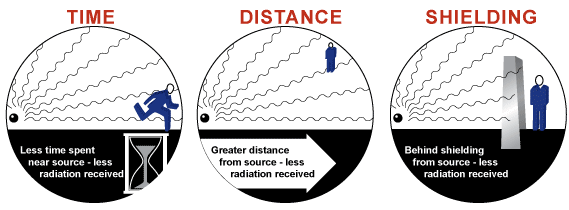
\includegraphics[scale=0.5]{img/TimeDistShield.png}
  \caption{Time Dist Shield}
  \label{fig:TimeDistShield}
\end{figure}
\subsection{Zeit}
Die Strahlungsdosis ist direkt proportional zu der Zeit, die in der Strahlung verbracht wird. Daher sollte sich eine Person nicht länger als nötig in der Nähe einer Strahlungsquelle aufhalten. Wenn ein Vermessungsgerät 4 mR / h an einem bestimmten Ort liest, wird eine Gesamtdosis von 4mR erhalten, wenn eine Person für eine Stunde an diesem Ort verbleibt. In einer zweistündigen Zeitspanne würde eine Dosis von 8 mR erhalten werden. Die folgende Gleichung kann verwendet werden, um eine einfache Berechnung durchzuführen, um die Dosis zu bestimmen, die in einem Strahlungsgebiet empfangen wird oder wurde.\\
Dose = Dose Rate x Time \\
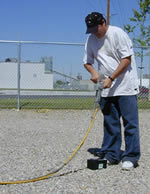
\includegraphics[scale=0.7]{img/timeDist.jpg}\\
Bei Verwendung einer Gammakamera ist es wichtig, die Quelle von der abgeschirmten Kamera so schnell wie möglich zum Kollimator zu bringen, um die Expositionszeit der ungeschirmten Quelle zu begrenzen. Vorrichtungen, die Strahlung in einigen Richtungen abschirmen, aber in einer oder mehreren anderen Richtungen passieren können, sind als Kollimatoren bekannt. Dies wird in den Bildern am Ende dieser Seite veranschaulicht.
\subsubsection{Beispielrechnungen 1}
Ein Techniker befindet sich in einem Bereich für 10 Minuten und der Messwert auf dem Vermessungsmesser beträgt 5 mR / h. Welche Strahlendosis erhält der Techniker?\\
5mR/h / 60 min./h = 0.0833 mR/min.\\
0.0833 mR/min. x 10 min = 0.833 mR  total dose.\\

\subsubsection{Beispielrechnungen 2}
Ein Techniker möchte unter Berücksichtigung der oben genannten Bedingungen nicht mehr als eine Dosis von 1,0 mR erhalten. Wie lange kann der Techniker maximal in der Gegend bleiben?\\
1.0 mR / 0.0833 mR/min. = 12 min \\
Die berechneten Dosierungen wären Annäherungen. Die tatsächlichen Dosierungen können aufgrund von Streuung und anderen Überlegungen variieren. Die TLD oder das Film-Badge sollte verwendet werden, um die von einer Person erhaltene Dosis zu bestimmen.
\subsection{Entfernung}
Die zunehmende Entfernung von der Strahlungsquelle verringert die Menge der empfangenen Strahlung. Wenn Strahlung von der Quelle ausgeht, breitet sie sich aus und wird weniger intensiv.\\
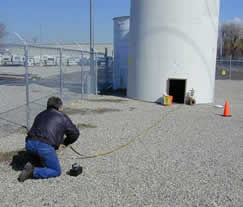
\includegraphics[scale=0.5]{img/distance.jpg}\\
Dies ist vergleichbar mit dem Stehen in der Nähe eines Feuers. Je näher eine Person dem Feuer steht, desto intensiver fühlt sich die Hitze vom Feuer an. Dieses Phänomen kann durch eine Gleichung ausgedrückt werden, die als das umgekehrte quadratische Gesetz bekannt ist, das besagt, dass, wenn sich die Strahlung von der Quelle ausbreitet, die Dosierung umgekehrt zum Quadrat der Entfernung abnimmt.\\
Berechnung der Intensität mit dem inversen Quadratgesetz: \\

\( \frac {I1}  {I2} = \frac {D2^2} { D1^2} \) \\
\\
I1 = Intensität 1 bei D1 \\
I2 = Intensität 2 bei D2 \\
D1 = Entfernung 1 von der Quelle\\
D2 = Entfernung 2 von der Quelle\\

\subsubsection{Beispielrechnungen 1}
Die Strahlungsintensität beträgt 530 U / h bei 5 Fuß Entfernung von einer Quelle. 
Wie groß ist die Intensität der Strahlung bei 10 Fuß?
Überarbeiten Sie die Gleichung, um die Intensität in Entfernung 2 zu lösen:\\
\( I2 = I1*\frac{D1^2} { D2^2} \) \\
Stecken Sie die bekannten Werte ein\\
\( I2 = 530R/h * \frac{(5ft)^2} {(10ft)^2} \) \\

Löse für I2= 132.5 R/h \\
In diesem Fall wurde die Entfernung verdoppelt und die Intensität an diesem Punkt hat sich um den Faktor vier verringert.

\subsubsection{Beispielrechnungen 2}
Eine Quelle erzeugt eine Intensität von 456 R / h bei einem Fuß von der Quelle. Wie groß wäre der Abstand in Fuß zu den 100, 5 und 2 mR / h Grenzen.\\
Konvertiere R / Stunde in mR / Stunde\\
456R/h * 1000 = 456,000 mR/h\\
\big (\ D2 = $\sqrt[\leftroot{3}\uproot{3}]{\tfrac{I1*D1^2}{I2}}$  \big) -----> \Big(
\ D2 = $\sqrt[\leftroot{3}\uproot{3}]{\tfrac{456,000 mR/h * (1ft)^2}{100 mR/h}}$ \Big) ---> \Bigg(D2= 67.5 \Bigg) 
\subsection{Abschirmung}
Der dritte Weg, die Strahlenexposition zu reduzieren, besteht darin, etwas zwischen dem Radiographen und der Strahlungsquelle zu platzieren. Im Allgemeinen gilt, je dichter das Material ist, desto mehr Abschirmung wird es bereitstellen. Die wirksamste Abschirmung wird durch Metall aus abgereichertem Uran erreicht. Es wird hauptsächlich in Gammastrahlenkameras wie der unten gezeigten verwendet.\\
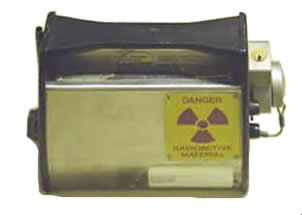
\includegraphics[scale=0.9]{img/cameraoutside.jpg} 
 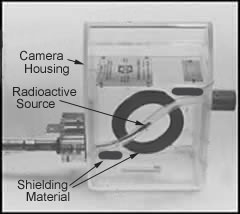
\includegraphics[scale=0.5]{img/camera_pigtail.jpg}\\
Der Kreis aus dunklem Material in der Plastik-Durchsichtskamera (unten rechts) wäre tatsächlich eine Kugel aus abgereichertem Uran in einer echten Gammastrahlenkamera. Abgereichertes Uran und andere Schwermetalle, wie Wolfram, sind sehr wirksam bei der Abschirmung von Strahlung, da ihre dicht gepackten Atome es der Strahlung schwer machen, sich durch das Material zu bewegen, ohne mit den Atomen in Wechselwirkung zu treten. Blei und Beton sind die am häufigsten verwendeten Strahlenschutzmaterialien, hauptsächlich weil sie einfach zu verarbeiten sind und leicht verfügbar sind. Beton wird häufig bei der Konstruktion von Strahlungsgewölben verwendet. Einige Gewölbe werden auch mit Bleifolien verkleidet, um die Strahlung auf ein akzeptables Maß von außen zu reduzieren.

\begin{figure}[htb]
\centering
  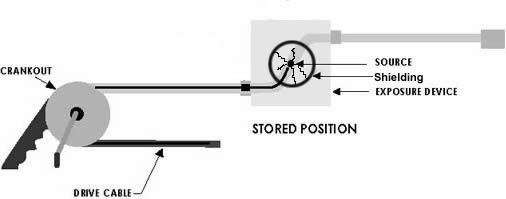
\includegraphics[scale=0.4]{img/Gamma1.jpg}
  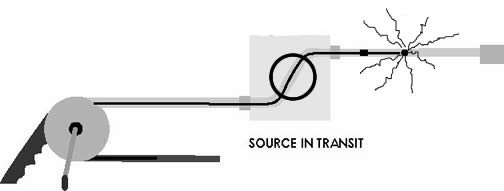
\includegraphics[scale=0.4]{img/Gamma2.jpg}
  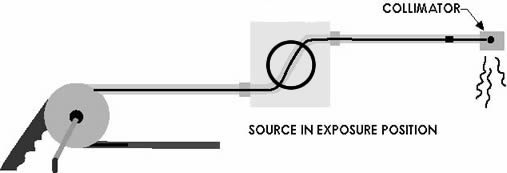
\includegraphics[scale=0.4]{img/Gamma3.jpg}
  \caption{Camera}
  \label{fig:Camera}
\end{figure}
\section{Sicherheitskontrollen}
\label{kontrollen}
Da Röntgen- und Gammastrahlung von den menschlichen Sinnen nicht wahrgenommen werden können und der daraus resultierende Schaden für den Körper nicht unmittelbar ersichtlich ist, wird eine Vielzahl von Sicherheitskontrollen verwendet, um die Exposition zu begrenzen. Die zwei grundlegenden Arten von Strahlenschutzkontrollen, die für eine sichere Arbeitsumgebung verwendet werden, sind technische und administrative Kontrollen. Engineered Kontrollen umfassen Abschirmung, Verriegelungen, Alarme, Warnsignale und Materialeinschließung. Administrative Kontrollen umfassen Buchungen, Prozeduren, Dosimetrie und Schulungen.
\subsection{Engineered Kontrollen}
Engineered Kontrollen wie Abschirmung und Türverriegelungen werden benutzt, um die Strahlung in einem Kabinett oder in einem "Strahlungsgewölbe" zu enthalten.
Feste Abschirmungsmaterialien sind üblicherweise Beton und / oder Blei mit hoher Dichte. Türverriegelungen werden verwendet, um den Strom zu Röntgenstrahlen erzeugenden Geräten sofort zu unterbrechen, wenn eine Tür versehentlich geöffnet wird, wenn Röntgenstrahlen erzeugt werden. Warnlichter werden verwendet, um Arbeiter und die Öffentlichkeit darauf aufmerksam zu machen, dass Strahlung verwendet wird. Sensoren und Warnalarme werden oft verwendet, um zu signalisieren, dass eine vorbestimmte Menge an Strahlung vorhanden ist. Sicherheitskontrollen sollten niemals manipuliert oder umgangen werden.\\
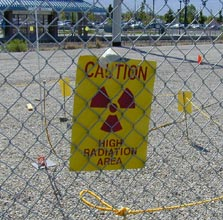
\includegraphics[scale=0.9]{img/safetyshild.jpg}\\
Wenn eine tragbare Radiographie durchgeführt wird, ist es meistens nicht praktikabel, Alarm- oder Warnlichter im Belichtungsbereich zu platzieren. Seile und Schilder werden verwendet, um den Zugang zu Strahlungsbereichen zu blockieren und die Öffentlichkeit auf das Vorhandensein von Strahlung aufmerksam zu machen. Gelegentlich verwenden Radiografen batteriebetriebene Blitzlichter, um die Öffentlichkeit auf das Vorhandensein von Strahlung aufmerksam zu machen. Tragbare oder temporäre Abschirmvorrichtungen können aus Materialien oder Geräten hergestellt werden, die sich im Bereich der Inspektion befinden. Zur vorübergehenden Abschirmung können Stahlbleche, Stahlträger oder andere Geräte verwendet werden. Es liegt in der Verantwortung des Radiografen, den Absorptionswert verschiedener Materialien zu kennen und zu verstehen. Weitere Informationen zu Absorptionswerten und Materialeigenschaften finden Sie im Röntgenbereich dieser Website.
\subsection{Verwaltungskontrollen}
Wie bereits erwähnt, ergänzen administrative Kontrollen die technischen Kontrollen. Diese Steuerelemente umfassen Buchungen, Prozeduren, Dosimetrie und Training. In der Regel ist es erforderlich, dass alle Bereiche, in denen röntgenstrahlerzeugende Geräte oder radioaktive Materialien enthalten sind, mit Schildern versehen sind, auf denen das Strahlungssymbol und ein Hinweis auf die Gefahren der Strahlung angebracht sind. Normale Betriebsverfahren und Notfallverfahren müssen ebenfalls vorbereitet und befolgt werden. In den USA schreibt das Bundesgesetz vor, dass jede Person, die wahrscheinlich mehr als 10\% eines jährlichen Arbeitsplatzgrenzwerts erhält, auf Strahlenbelastung überwacht wird. Diese Überwachung wird durch den Einsatz von Dosimetern erreicht, die im Abschnitt Strahlungssicherheitsausrüstung dieses Materials behandelt werden. Eine gute Schulung mit begleitender Dokumentation ist auch eine sehr wichtige administrative Kontrolle.

\subsection{Strahlenschutzbereiche}
Strahlenschutzgebiete werden bei Tätigkeiten eingerichtet, für die eine Genehmigung nach den nationalen Strahlenschutzgesetzen erforderlich ist. Je nach Strahlenexposition wird zwischen Überwachungsbereichen, Kontrollbereich und Sperrbereich hinsichtlich der externen und internen Strahlenexposition unterschieden. Überall dort, wo EU-Vorschriften gelten, gelten folgende Werte:\\
\\
{\rowcolors{3}{yellow}{green}
\begin{tabular}{ |p{2.5cm}|p{4cm}|p{4cm}|  }
\hline
\multicolumn{3}{|c|}{Strahlenschutzbereiche} \\
\hline
Isotop Quelle& Sperrbereich &Kontrollbereich \\
\hline
Iridium192 &1.6 $\sqrt{Aktivität}$&14 $\sqrt{Aktivität}$\\
\hline
Cobalt 60&2.6 $\sqrt{Aktivität}$&23 $\sqrt{Aktivität}$ \\
\hline
Cesium 137&1.3 $\sqrt{Aktivität}$& 11.5 $\sqrt{Aktivität}$\\
\hline
Ytterbium169&0.8 $\sqrt{Aktivität}$&7 $\sqrt{Aktivität}$ \\
\hline
\end{tabular} \\
\subsubsection{Überwachungsbereich}
Überwachungsbereiche sind die Bereiche, in denen Personen eine höhere effektive Dosis als 1 mSv oder höhere Organdosen als 15 mSv für die Augenlinse oder 50 mSv für die Haut, die Hände, die Unterarme, die Füße und Knöchel im Kalenderjahr erhalten können. Oft wird das gesamte Betriebsgelände als Überwachungsbereich betrachtet und (zum Beispiel bei Kernkraftwerken) durch einen Zaun oder ähnliche Maßnahmen vom allgemeinen Staatsgebiet abgetrennt.
\subsubsection{Kontrollbereich}
Der Kontrollbereich ist meist vom Überwachungsbereich umschlossen. In ihm können Personen eine effektive Dosis von mehr als 6 mSv pro Kalenderjahr oder höhere Organdosen als 45 mSv pro Kalenderjahr für die Augenlinse oder 150 mSv pro Kalenderjahr für die Haut, die Hände, die Unterarme, die Füße und Knöchel erhalten. Kontrollbereiche müssen abgegrenzt und deutlich sichtbar gekennzeichnet sein. Ein Kontrollbereich darf nur zur Durchführung oder Aufrechterhaltung der vorgesehenen Betriebsvorgänge betreten werden. Besucher haben nur mit behördlicher Erlaubnis Zutritt. Bei Personen, die sich im Kontrollbereich aufhalten, müssen die Körperdosen bestimmt werden – üblicherweise mit einem amtlichen Dosimeter. Vor dem erstmaligen Zutritt und dann mindestens jährlich muss eine Unterweisung insbesondere über die anzuwendenden Strahlenschutzmaßnahmen durchgeführt werden.

\subsubsection{Sperrbereich}
Sperrbereiche sind Bereiche innerhalb eines Kontrollbereichs, in denen die Ortsdosisleistung höher als 3 mSv pro Stunde sein kann. Personen darf der Aufenthalt in einem Sperrbereich nur erlaubt werden, wenn sie unter der Aufsicht einer beauftragten fachkundigen Person zur Durchführung vorgesehener Betriebsvorgänge oder aus zwingendem Grund tätig werden müssen. Sperrbereiche sind abzugrenzen und deutlich sichtbar zu kennzeichnen.
Der Zutritt zu Strahlenschutzbereichen ist nicht frei. Einschränkungen finden sich z. B.in der deutschen StrlSchV (§ 37 Zutritt zu Strahlenschutzbereichen) für Überwachungs-, Kontroll- und Sperrbereiche.
Für alle übrigen Bereiche eines Betriebes, die nicht Strahlenschutzbereiche sind, gilt der Grenzwert für das allgemeine Staatsgebiet für die Ortsdosisleistung von 1 mSv pro Jahr.
\begin{figure}[htb]

  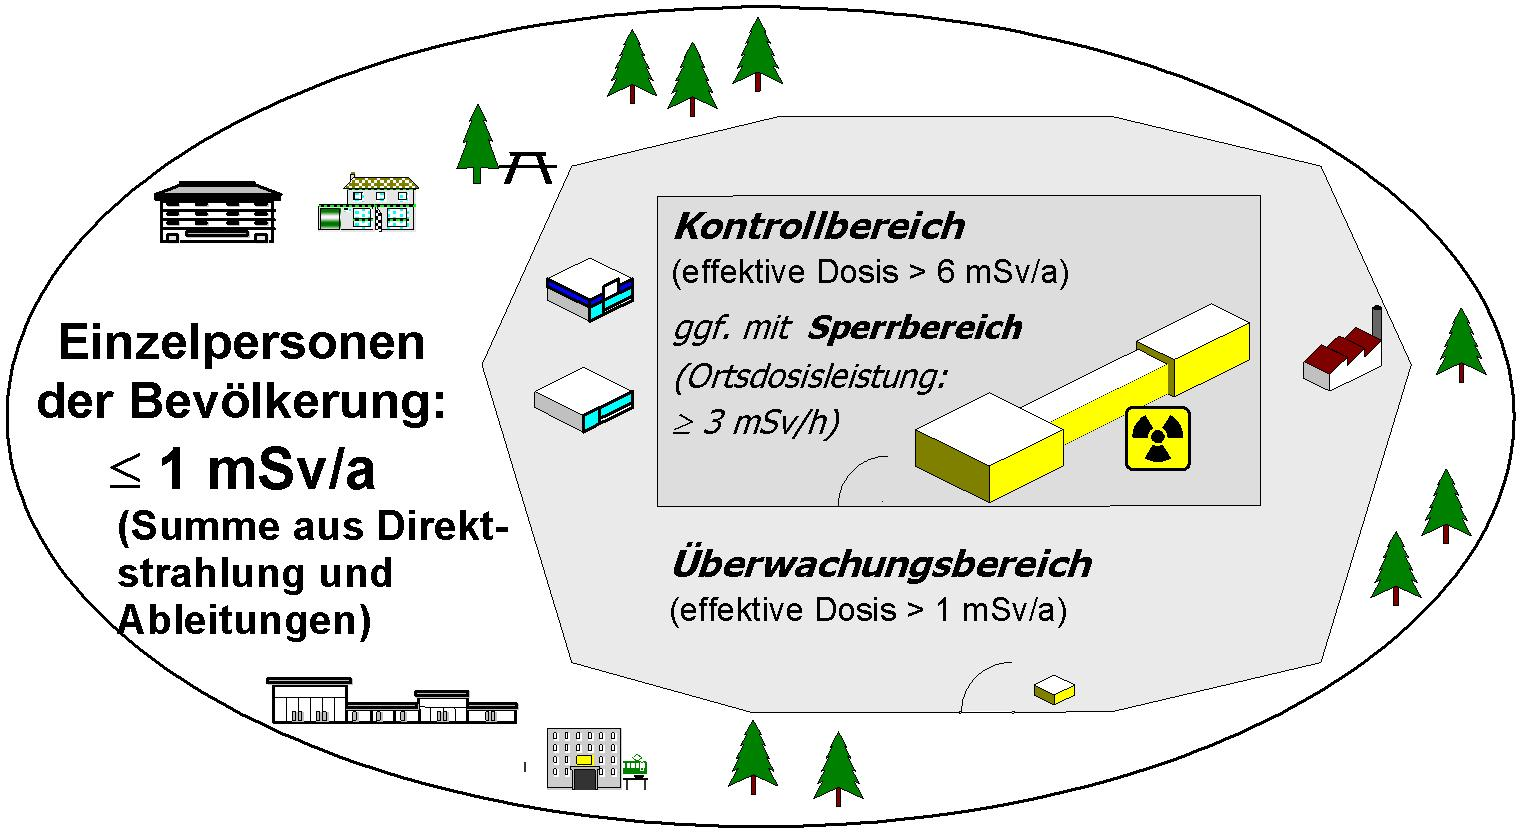
\includegraphics[scale=0.4]{img/Strahlenschutzbereiche.jpg}
  \caption{Strahlenschutzbereiche}
  \label{fig:Strahlenschutzbereiche}
\end{figure}


\section{Verantwortlichkeiten}
Der sichere Umgang mit der Strahlung liegt in der Verantwortung aller, die an der Verwendung und Verwaltung von strahlungserzeugenden Geräten und Materialien beteiligt sind. Abhängig von der Größe der Organisation können bestimmte Verantwortlichkeiten verschiedenen Personen und / oder Ausschüssen zugewiesen werden.
\subsection{Strahlenschutzbeauftragter "Radiation Safety Officer"(RSO)}

Alle Organisationen, die zur Verwendung ionisierender Strahlung zugelassen sind, müssen über einen Strahlenschutzbeauftragten verfügen. Der RSO ist die vom Unternehmen autorisierte Person, die als Ansprechpartner für alle Aktivitäten dient, die im Rahmen der Genehmigung durchgeführt werden. Der RSO stellt sicher, dass Strahlenschutzaktivitäten in Übereinstimmung mit genehmigten Verfahren und regulatorischen Anforderungen durchgeführt werden. Einige der gemeinsamen Verantwortlichkeiten für den RSO sind:\\
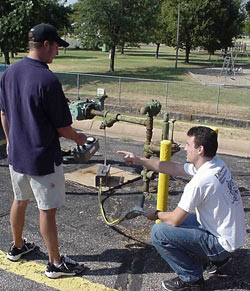
\includegraphics[scale=0.7]{img/rso.jpg}\\
\begin{enumerate}
  \item Sicherstellen, dass alle Personen, \\die Strahlengeräte verwenden, angemessen geschult     und beaufsichtigt werden.
  \item Sicherstellen, dass alle Personen, \\die das Gerät benutzen, formell zur Verwendung des Geräts autorisiert wurden.
  \item Sicherstellen, dass alle Regeln, \\Vorschriften und Verfahren für den sicheren Umgang mit  radioaktiven Quellen und Röntgensystemen eingehalten werden.
  \item Sicherstellen, dass geeignete Betriebs,Notfall- und ALARA-Verfahren \\entwickelt wurden und allen Systembenutzern zur Verfügung stehen.
  \item Sicherstellen, dass genaue Aufzeichnungen \\ über die Verwendung der Quellen und Geräte erhalten bleiben.
  \item Sicherstellen, dass die erforderlichen Strahlungsuntersuchungen und Dichtigkeitsprüfungen durchgeführt und dokumentiert werden.
  \item Sicherstellen, dass Systeme und Geräte vor unbefugtem Zugriff oder Entfernung geschützt sind.
\end{enumerate}
Die Mindestqualifikationen, Schulungen und Erfahrungen für RSOs für die industrielle Radiographie sind wie folgt: (1) Abschluss der Trainings- und Testanforderungen von Sec. 34.43 (a) von Teil 10 des Federal Code of Regulations, (2) 2000 Stunden praktische Erfahrung als qualifizierte Radiotechniker in industriellen radiographischen Operationen, und (3) Formale Ausbildung in der Einrichtung und Wartung eines Strahlenschutzprogramms.
\subsection{Strahlenschutzausschuss "Radiation Safety Committee" (RSC)}
Einige Organisationen haben möglicherweise einen Strahlenschutzausschuss (RSC), der den RSO unterstützt. Das RSC überwacht häufig die Richtlinien, Verfahren und Verantwortlichkeiten eines Strahlenschutzprogramms eines Unternehmens.
\subsection{Systembenutzer}
Die zur Verwendung des röntgenstrahlerzeugenden Systems oder der Gammaquellen autorisierten Personen sind dafür verantwortlich, dass :
\begin{enumerate}
\item Alle Regeln, Vorschriften und Verfahren zur sicheren Verwendung des Röntgensystems werden befolgt.
\item Eine genaue Aufzeichnung der Verwendung des Systems wird aufrechterhalten.
\item Alle Sicherheitsprobleme mit dem System werden dem RSO gemeldet und vor der weiteren Verwendung korrigiert.
\item Das System ist vor unbefugtem Zugriff oder Entfernung geschützt.
\end{enumerate}
\subsection{Verfahren}
Schriftliche Arbeitsanweisungen müssen entwickelt und jedem zur Verfügung gestellt werden, der mit Strahlenquellen oder röntgenstrahlenden Geräten arbeitet. Diese Verfahren müssen für die Ausrüstung und ihre Verwendung in einer bestimmten Anwendung spezifisch sein. Den Beschäftigten die Bedienungsanleitung des Geräteherstellers einfach zur Verfügung zu stellen, genügt dieser Anforderung nicht. Das Betriebsverfahren muss jederzeit befolgt werden, es sei denn, es liegt eine schriftliche Genehmigung des Strahlenschutzbeauftragten vor.
\subsubsection{Standardablauf}
Die Betriebsanweisungen müssen mindestens Anweisungen für Folgendes enthalten:
\begin{enumerate}
\item Angemessene Handhabung und Verwendung lizenzierter umschlossener Strahlenquellen und radiographischer Expositionsgeräte, so dass keine Person Strahlenexpositionen ausgesetzt ist, die über den festgelegten Expositionsgrenzwerten liegen.
\item Methoden und Anlässe für die Durchführung von Strahlungsuntersuchungen.
\item Methoden zur Kontrolle des Zugangs zu Radiographiebereichen.
\item Methoden und Anlässe zum Sichern und Sichern von Röntgengeräten, Transport- und Lagerbehältern und versiegelten Quellen.
\item Personalüberwachung und Einsatz von Personalüberwachungsgeräten.
\item Transport von versiegelten Quellen zu Feldstandorten, einschließlich Verpackung radiographischer Expositionsgeräte und Lagerbehälter in den Fahrzeugen, Plakatierung von Fahrzeugen bei Bedarf und Kontrolle der versiegelten Quellen während des Transports.
\item Überprüfung, Wartung und Funktionsfähigkeitsprüfung von Röntgengeräten, Vermessungsinstrumenten, Transportbehältern und Lagerbehältern.
\item Das Verfahren zur Identifizierung und Meldung von Mängeln und Nichteinhaltung.
\item Wartung von Aufzeichnungen.

\end{enumerate}

\subsubsection{Notfallmaßnahmen}
Es müssen auch Verfahren entwickelt werden, die die Mitarbeiter im Notfall leiten. Einige der Elemente, die abgedeckt werden könnten, sind:
\begin{enumerate}
\item Schritte, die sofort von dem Radiographiepersonal ergriffen werden müssen, wenn festgestellt wird, dass ein Taschendosimeter außerhalb der Skala liegt oder ein Alarmratenmesser unerwartet alarmiert.
\item Schritte zur Minimierung der Exposition von Personen im Falle eines Unfalls.
\item Das Verfahren zur Benachrichtigung der richtigen Personen im Falle eines Unfalls.
\item Wiederherstellungsprozedur für radioaktive Quellen, wenn der Lizenznehmer die Wiederherstellung durchführt.

\end{enumerate}
\subsection{Umfragetechnik}
Die Mehrheit der Überbelichtungen in der industriellen Radiographie ist das Ergebnis dessen, dass der Radiograf den Ort eines Gammastrahlers nicht kennt und keine geeignete Strahlungserhebung durchführt.
Expositionsgewölbe sind mit Warnleuchten und Sicherheitsverriegelungsschaltern ausgestattet, die eine Sicherheitsmarge für die Arbeiter bieten. Es muss gelegentlich eine Untersuchung durchgeführt werden, um sicherzustellen, dass in den Tresoren keine Strahlung austritt und dass die Sicherheitsvorrichtungen ordnungsgemäß funktionieren. Wenn jedoch eine Radiographie mit Gammastrahlern im Feld durchgeführt wird, muss sich der Röntgengeräteher stark auf Messungen mit einem Vermessungsmeter verlassen, da andere Sicherheitsvorrichtungen nicht üblich sind. Eine Reihe von Erhebungen muss durchgeführt werden, und einige der Ergebnisse dieser Erhebungen müssen dokumentiert werden, wenn mit Gammastrahlern im Feld transportiert und gearbeitet wird.
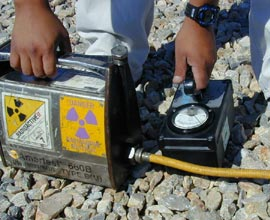
\includegraphics[scale=0.9]{img/cameraTest.jpg}\\
\subsubsection{Annäherung an das Belichtungsgerät}
Ein Techniker sollte sich gründlich mit dem Betrieb eines Vermessungsmessers auskennen, da der bestimmungsgemäße Gebrauch des Geräts unerlässlich ist. Bevor das Belichtungsgerät (Kamera) aus dem Speicher genommen wird, muss die Kalibrierung des Vermessungszählers überprüft und der Batteriestand überprüft werden. Wenn Sie sich dem Belichtungsgerät nähern, um es vom Lagerort zu entfernen, sollte das Vermessungsgerät griffbereit und betriebsbereit sein. Der Vermessungsmesser sollte neben dem Belichtungsgerät platziert werden, um zu überprüfen, ob die Quelle im Projektor enthalten ist, und um sicherzustellen, dass das Vermessungsgerät ordnungsgemäß funktioniert. Vermessungszählerstände sollten mit früheren Messungen verglichen und aufgezeichnet werden.
\subsubsection{Transport des Belichtungsgeräts}
Wenn das Belichtungsgerät transportiert wird, muss es sicher im Fahrzeug verstaut werden. Eine verschließbare Metallbox ist oft im Heck des Fahrzeugs verschraubt. Ein Überblick über die Überverpackung, die Außenseite des Fahrzeugs und den Fahrerraum wird dann durchgeführt und dokumentiert.
\subsubsection{Vorbereitung auf eine Exposition}
Auf der Baustelle wird der Expositionsbereich bewertet, Abstandsberechnungen für die Begrenzung der Sperrzonen und Seile und Schilder, die entsprechend platziert werden, durchgeführt. Sobald dies abgeschlossen ist, ist der Röntgentechniker bereit, das Belichtungsgerät aus seinem Ablagefach im Fahrzeug zu entfernen. Der Vermessungszähler sollte überwacht werden, wenn das Aufbewahrungsfach angefahren wird und wenn das Expositionsgerät aus dem Fach entfernt wird. Tägliche Sicherheitskontrollen sollten dann durchgeführt werden. Sobald diese Überprüfungen abgeschlossen sind, können der Röntgenassistent und der Assistent das Belichtungsgerät zum Expositionsort bewegen. Da die Kurbeln und Führungsrohre zur Vorbereitung der ersten Exposition angebracht sind, sollte das Vermessungsgerät überwacht werden. Bevor die Quelle freigelegt wird, sollte der Assistent den Bereich auf Personen überprüfen, die möglicherweise in den eingeschränkten Bereich eingedrungen sind, und sich dann außerhalb der Seilgrenze bewegen.
\subsubsection{Eine Belichtung erledigen}

Der Röntgentechniker sollte sich in der maximalen Entfernung von der Belichtungsvorrichtung befinden, die das Führungsrohr erlaubt, wenn er oder sie die Quelle schnell aus der Belichtungsvorrichtung herausritzt und einrastet. Wenn sich die Quelle aus dem Belichtungsgerät bewegt, wird der Vermessungsmesser auf ein sehr hohes Niveau ansteigen und sich dann verringern, sobald sich die Quelle innerhalb des Kollimators befindet. Während der Exposition wird der Assistent die festgelegte Grenze überwachen, um die vorhandenen Strahlungswerte zu bestimmen. Wenn der Vermessungsmesser anzeigt, dass die Werte höher als berechnet sind, muss die Grenze erweitert werden.
\subsubsection{Die Quelle zurückziehen}
Beim Zurückziehen der Quelle sehen die Röntgenphotographen einen Anstieg der Messwerte, wenn sich die Quelle aus dem Kollimator bewegt und in den Projektor zurückgezogen wird. Wenn sich die Quelle innerhalb des Belichtungsgeräts befindet, sollte sich der Röntgentechniker ihm nähern, während er den Vermessungsmesser überwacht. Wenn die Quelle ordnungsgemäß eingefahren ist, sollte bei Annäherung an das Belichtungsgerät keine Erhöhung des Messgeräts angezeigt werden. Das Belichtungsgerät sollte von allen Seiten beobachtet werden, wobei besonders auf die Vorderseite des Geräts zu achten ist. Die gesamte Länge des Führungsrohrs muss dann vermessen werden.

Dieser Vorgang wird für jede Belichtung wiederholt. Die Ergebnisse der Untersuchung müssen dokumentiert werden, wenn das Expositionsgerät zum Transport an das Fahrzeug zurückgegeben wird und wenn es an seinen Lagerort zurückgebracht wird.\\
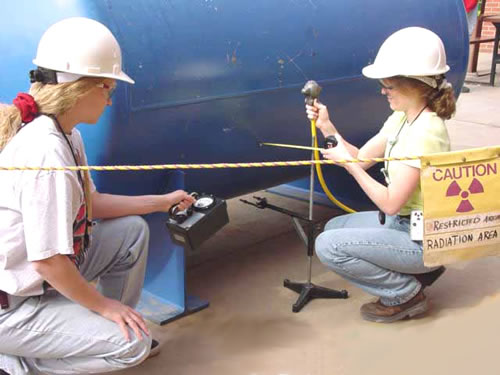
\includegraphics[scale=0.7]{img/isotope-radiography-pressure-vessel.jpg}\\
\subsection{Strahlungsdetektoren}
Instrumente zur Strahlungsmessung fallen in zwei große Kategorien:
\begin{itemize}
\item Messgeräte 
\item Persönliche Dosismessgeräte. 
\end{itemize}
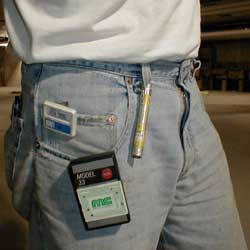
\includegraphics[scale=0.5]{img/strahlungsdetektor.jpg}\\
\\
Frequenzmessgeräte messen die Rate, mit der die Belichtung empfangen wird 
(häufiger als Strahlungsintensität bezeichnet).
Vermessungszähler, akustische Alarme und Bereichsüberwachungsgeräte fallen in diese Kategorie. Diese Instrumente zeigen eine Strahlungsintensitätsablesung relativ zur Zeit, wie etwa R / h oder mR / h. Eine Analogie kann zwischen diesen Instrumenten und dem Tachometer eines Autos hergestellt werden, da beide Messeinheiten relativ zur Zeit sind.
Dosismessgeräte sind solche, die den Gesamtbetrag der während eines Messzeitraums erhaltenen Exposition messen. Die Dosimeter oder Dosimeter, die üblicherweise in der industriellen Radiographie verwendet werden, sind kleine Vorrichtungen, die dazu bestimmt sind, von einer Person getragen zu werden, um die von der Person empfangene Exposition zu messen. Eine Analogie kann zwischen diesen Instrumenten und dem Kilometerzähler eines Autos hergestellt werden, da beide akkumulierte Einheiten messen.

\subsection{Messgeräte}
Der Vermessungsmesser ist die wichtigste Ressource, die ein Röntgentechniker benötigt, um die Anwesenheit und Intensität der Strahlung zu bestimmen. Eine Überprüfung der Vorfall- und Überbelichtungsberichte zeigt, dass ein Großteil dieser Art von Ereignissen aufgetreten ist, wenn ein Techniker kein Vermessungsinstrument verwendet hat oder nicht verwendet hat.\\
Zur Messung der Strahlung im Feld stehen viele verschiedene Modelle von Vermessungszählern zur Verfügung. Sie alle bestehen im Wesentlichen aus einem Detektor und einer Ausleseanzeige. Analoge und digitale Anzeigen sind verfügbar. Die meisten Vermessungsmesser, die für die industrielle Radiographie verwendet werden, verwenden einen gasgefüllten Detektor.\\
\begin{figure}[htb]
  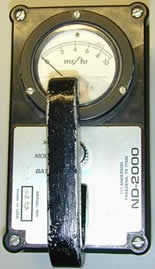
\includegraphics[scale=0.5]{img/radiometer.jpg}
  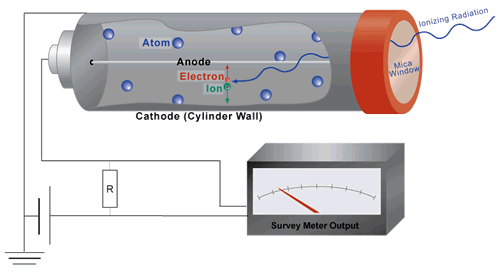
\includegraphics [scale=0.5]{img/radiometer_technik.png}
  \caption{Radiometer}
  \label{fig:radiometer}
\end{figure}
Gasgefüllte Detektoren bestehen aus einem gasgefüllten Zylinder mit zwei Elektroden. Manchmal wirkt der Zylinder selbst als eine Elektrode, und eine Nadel oder ein dünner straff gespannter Draht entlang der Achse des Zylinders wirkt als die andere Elektrode. Eine Spannung wird an die Vorrichtung angelegt, so dass die zentrale Nadel oder der Draht eine Anode (+ Ladung) wird und die andere Elektrode oder Zylinderwand die Kathode (- Ladung) wird. Das Gas wird ionisiert, sobald der Zähler in die Nähe von radioaktiven Substanzen gebracht wird. Das elektrische Feld, das durch die Potentialdifferenz zwischen der Anode und der Kathode erzeugt wird, bewirkt, dass sich die Elektronen jedes Ionenpaars zur Anode bewegen, während das positiv geladene Gasatom zur Kathode gezogen wird. Dies führt zu einem elektrischen Signal, das verstärkt wird, mit der Belichtung korreliert und als Wert angezeigt wird.\\
Abhängig von der zwischen der Anode und der Kathode angelegten Spannung kann der Detektor als eine Ionenkammer, ein Proportionalzähler oder ein Geiger-Müller (GM) -Detektor betrachtet werden. Jeder dieser Detektortypen hat seine Vor- und Nachteile. Eine kurze Zusammenfassung jedes dieser Detektoren folgt.
\subsubsection{Ionenkammerzähler}
Ionenkammern haben eine relativ niedrige Spannung zwischen der Anode und der Kathode, was zu einer Ansammlung von nur den Ladungen führt, die bei dem anfänglichen Ionisationsereignis erzeugt werden. Diese Art von Detektor erzeugt ein schwaches Ausgangssignal, das der Anzahl der Ionisationsereignisse entspricht. Höhere Energien und Strahlungsintensitäten erzeugen mehr Ionisierung, was zu einer stärkeren Ausgangsspannung führt.\\
Die Sammlung von nur primären Ionen liefert Informationen über die tatsächliche Strahlenbelastung (Energie und Intensität). Die Messgeräte benötigen jedoch eine empfindliche Elektronik, um das Signal zu verstärken, was sie ziemlich teuer und empfindlich macht. Der zusätzliche Aufwand und die erforderliche Sorgfalt sind gerechtfertigt, wenn genaue Strahlenexpositionsmessungen über einen Bereich von Strahlungsenergien durchgeführt werden müssen. Dies könnte notwendig sein, wenn die von einem Röntgengenerator erzeugte Bremsstrahlungsstrahlung gemessen wird. Ein Ionenkammer-Vermessungsmesser wird manchmal bei der Durchführung von Gammaradiographie im Feld verwendet, da es genaue Expositionsmessungen ungeachtet des verwendeten radioaktiven Isotops liefert.
\subsubsection{Proportionaler Zähler}
Proportionalzähldetektoren verwenden eine etwas höhere Spannung zwischen der Anode und der Kathode. Aufgrund des starken elektrischen Feldes werden die Ladungen, die bei der anfänglichen Ionisierung erzeugt werden, schnell genug beschleunigt, um andere Elektronen im Gas zu ionisieren. Die Elektronen, die in diesen sekundären Ionenpaaren erzeugt werden, sammeln zusammen mit den Primärelektronen weiterhin Energie, wenn sie sich zur Anode hin bewegen, und erzeugen dabei mehr und mehr Ionisationen. Das Ergebnis ist, dass jedes Elektron von einem primären Ionenpaar eine Kaskade von Ionenpaaren erzeugt. Dieser Effekt wird als Gasvermehrung oder -verstärkung bezeichnet. In diesem Spannungsregime ist die Anzahl der durch sekundäre Wechselwirkungen freigesetzten Teilchen proportional zur Anzahl der Ionen, die von den vorbeilaufenden ionisierenden Teilchen erzeugt werden. Daher werden diese Gasionisationsdetektoren als Proportionalzähler bezeichnet.

Wie Ionenkammerdetektoren unterscheiden Proportionaldetektoren zwischen den Strahlungsarten. Sie erfordern jedoch eine sehr stabile Elektronik, die teuer und zerbrechlich ist. Proportionaldetektoren werden normalerweise nur in einer Laborumgebung verwendet.

\subsubsection{Geiger-Müller (GM) Zähler}
Geiger-Müller-Zähler arbeitet unter noch höheren Spannungen zwischen der Anode und der Kathode, üblicherweise im Bereich von 800 bis 1200 Volt. Wie der Proportionalzähler beschleunigt die hohe Spannung die Ladungen, die bei der anfänglichen Ionisierung erzeugt werden, zu der Stelle, an der sie genug Energie haben, um andere Elektronen im Gas zu ionisieren. Diese Kaskadierung von Ionenpaaren tritt jedoch viel stärker auf und setzt sich fort, bis der Zähler mit Ionen gesättigt ist. Dies alles geschieht in einem Bruchteil einer Sekunde und führt zu einem elektrischen Stromimpuls konstanter Spannung. Die Ansammlung der großen Anzahl von Sekundärionen in der GM-Region ist als eine Lawine bekannt und erzeugt einen großen Spannungsimpuls. Mit anderen Worten, die Größe des Stromimpulses ist unabhängig von der Größe des Ionisationsereignisses, das ihn erzeugt hat.\\
Die elektronische Schaltung eines GM-Zählers zählt und zeichnet die Anzahl der Impulse auf und die Information wird oft in Zählimpulsen pro Minute angezeigt. Wenn das Instrument einen Lautsprecher hat, können die Impulse auch ein hörbares Klicken erzeugen. Wenn das Gasvolumen in der Kammer vollständig ionisiert ist, stoppt die Ionensammlung, bis der elektrische Impuls entlädt. Auch dies dauert nur einen Bruchteil einer Sekunde, aber dieser Prozess begrenzt die Geschwindigkeit, mit der einzelne Ereignisse erkannt werden können.\\
Da sie individuelle ionisierende Ereignisse anzeigen können, sind GM-Zähler im Allgemeinen empfindlicher gegenüber niedrigen Strahlungswerten als Ionenkammerinstrumente. Mittels Kalibrierung kann die Zählrate als Belichtungsrate über einen bestimmten Energiebereich angezeigt werden. Wenn sie für die Gammaradiographie verwendet werden, werden GM-Messgeräte typischerweise für die Energie der verwendeten Gammastrahlung kalibriert. Meistens liefert Gammastrahlung von Cs-137 bei 0,662 MeV die Kalibrierung. Nur kleine Fehler treten auf, wenn der Röntgengerät Ir-192 (durchschnittliche Energie etwa 0,34 MeV) oder Co-60 (durchschnittliche Energie etwa 1,25 MeV) verwendet.\\
Da der Geiger-Müller-Zähler viel mehr Elektronen erzeugt als ein Ionenkammerzähler oder ein Proportionalzähler, erfordert er nicht die gleiche elektronische Perfektion wie andere Vermessungszähler. Dies führt zu einem relativ kostengünstigen und robusten Messgerät. Die Nachteile von GM-Messgeräten bestehen darin, dass sie nicht in der Lage sind, unterschiedliche Mengen an Ionisierung zu berücksichtigen, die durch unterschiedliche Photonen und nicht kontinuierliche Messungen verursacht werden (Entladen erforderlich).
\subsubsection{Vergleich von gasgefüllten Detektoren}
Die Grafik auf der rechten Seite zeigt die Beziehung der Ionensammlung in einem gasgefüllten Detektor gegenüber der angelegten Spannung. In dem Ionenkammerbereich ist die Spannung zwischen der Anode und der Kathode relativ niedrig und nur Primärionen werden gesammelt. In dem proportionalen Bereich ist die Spannung höher und Primärionen und eine Anzahl von Sekundärionen (proportional zu den ursprünglich gebildeten Primärionen) werden gesammelt. In der GM-Region wird eine maximale Anzahl von Sekundärionen gesammelt, wenn das Gas um die Anode vollständig ionisiert ist. Es sei angemerkt, dass eine Unterscheidung zwischen Strahlungsarten (E1 und E2) in der Ionenkammer und in Proportionalbereichen möglich ist. Strahlung auf verschiedenen Energieniveaus bildet eine unterschiedliche Anzahl von Primärionen im Detektor. In der GM-Region bleibt jedoch die Anzahl der pro Ereignis gesammelten Sekundärionen gleich, unabhängig von der Energie der Strahlung, die das Ereignis ausgelöst hat. Der GM-Zähler gibt die Fähigkeit auf, die Belichtung aufgrund verschiedener Strahlungsenergien im Austausch für einen großen Signalimpuls genau zu messen. Dieser große Signalimpuls vereinfacht die Elektronik, die für Instrumente wie Messgeräte benötigt wird.
\begin{figure}[htb]
\centering
  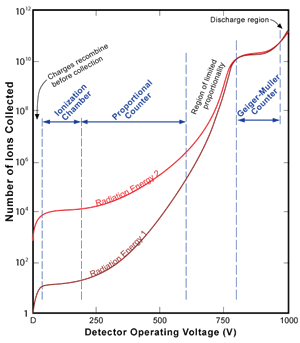
\includegraphics[scale=0.9]{img/detectorvoltage.png}
  \caption{detectorvoltage}
  \label{fig:detectorvoltage}
\end{figure}
\subsubsection{Taschen-Dosimeter}
Pocket-Dosimeter werden verwendet, um dem Träger eine sofortige Ablesung seiner Exposition gegenüber Röntgen- und Gammastrahlen zu ermöglichen. Wie der Name schon sagt, werden sie häufig in der Tasche getragen. Die beiden in der industriellen Radiographie gebräuchlichen Typen sind das Direct Read Pocket Dosimeter und das Digital Electronic Dosimeter.
\subsubsection{Direct Read Pocket Dosimeter}
Ein direkt lesendes Taschenionisationsdosimeter hat im Allgemeinen die Größe und Form eines Füllhalters. Das Dosimeter enthält eine kleine Ionisationskammer mit einem Volumen von ungefähr zwei Millilitern. In der Ionisationskammer befindet sich eine zentrale Drahtanode, und an dieser Drahtanode ist eine metallbeschichtete Quarzfaser befestigt. Wenn die Anode auf ein positives Potential geladen ist, wird die Ladung zwischen der Drahtanode und der Quarzfaser verteilt. Elektrostatische Abstoßung lenkt die Quarzfaser ab, und je größer die Ladung ist, desto größer ist die Ablenkung der Quarzfaser. Strahlung, die auf die Kammer einfällt, erzeugt eine Ionisierung innerhalb des aktiven Volumens der Kammer. Die durch Ionisation erzeugten Elektronen werden von der positiv geladenen zentralen Anode angezogen und gesammelt. Diese Ansammlung von Elektronen reduziert die positive Nettoladung und ermöglicht, dass die Quarzfaser in Richtung der ursprünglichen Position zurückkehrt. Die Menge der Bewegung ist direkt proportional zu der Menge der Ionisation, die auftritt.
\begin{figure}[htb]
  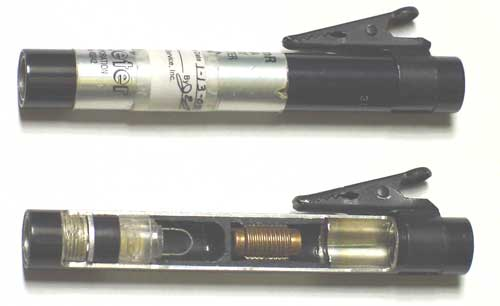
\includegraphics[scale=0.3]{img/dosimeter&cutaway.jpg}
  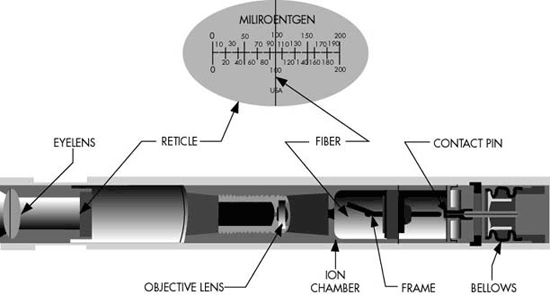
\includegraphics[scale=0.3]{img/dose.png}
  \caption{Pocket-Dosimeter}
  \label{fig:Pocket-Dosimeter}
\end{figure}

Indem das Instrument auf eine Lichtquelle gerichtet wird, kann die Position der Faser durch ein System von eingebauten Linsen beobachtet werden. Die Faser wird auf einer lichtdurchlässigen Skala betrachtet, die in Belichtungseinheiten abgestuft ist. Typische industrielle Röntgendiagnostik-Taschen-Dosimeter haben eine volle Skala von 200 Milliröntgen, aber es gibt Designs, die höhere Mengen aufzeichnen werden. Während der Schicht sollte der Dosimeterstand häufig überprüft werden. Die gemessene Exposition sollte am Ende jeder Schicht aufgezeichnet werden.
Der Hauptvorteil eines Taschendosimeters besteht in seiner Fähigkeit, dem Träger eine sofortige Ablesung seiner Strahlenbelastung zu ermöglichen. Es hat auch den Vorteil, wiederverwendbar zu sein. Die begrenzte Reichweite, die Unfähigkeit, eine dauerhafte Aufzeichnung zu liefern, und das Potenzial für Entlade- und Leseverluste aufgrund von Stürzen oder Stoßen sind einige der Hauptnachteile eines Taschendosimeters. Die Dosimeter müssen zu Beginn jeder Arbeitsschicht aufgeladen und aufgezeichnet werden. Ladungsverlust oder -drift können ebenfalls das Ablesen eines Dosimeters beeinflussen. Die Leckage sollte in einem Zeitraum von 24 Stunden nicht mehr als 2 Prozent des vollen Skalenwerts betragen.
\subsubsection{Digitales elektronisches Dosimeter}
Eine andere Art von Dosimeter ist das digitale Dosimeter. Diese Dosimeter zeichnen Dosisinformation und Dosisrate auf. Diese Dosimeter verwenden meistens Geiger-Müller-Zähler. Die Ausgabe des Strahlungsdetektors wird gesammelt, und wenn eine vorbestimmte Belichtung erreicht worden ist, wird die gesammelte Ladung entladen, um einen elektronischen Zähler auszulösen.
Der Zähler zeigt dann die akkumulierte Belichtung und Dosisrate in digitaler Form an.
Einige digitale elektronische Dosimeter enthalten eine akustische Alarmfunktion, die bei jeder aufgenommenen Belichtungsstufe ein akustisches Signal oder einen Piepton ausgibt. Einige Modelle können auch so eingestellt werden, dass ein kontinuierliches akustisches Signal ertönt, wenn eine voreingestellte Belichtung erreicht wurde. Dieses Format hilft, die Lesefehler zu minimieren, die mit direkt lesenden Taschenionisationskammer-Dosimetern verbunden sind, und ermöglicht es dem Instrument, eine höhere maximale Auslesung zu erreichen, bevor das Rücksetzen notwendig ist.
\begin{figure}[htb]
\centering
  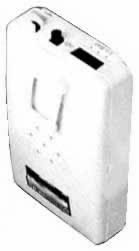
\includegraphics[scale=0.3]{img/Digital-Dosimeter.jpg}
  \caption{Pocket-Dosimeter}
  \label{fig:Pocket-Dosimeter}
\end{figure}
\subsubsection{Akustische Alarmgeräte Meter und digitale elektronische Dosimeter}
Akustische Alarme sind Geräte, die einen kurzen "Piep" oder "Chirp" abgeben, wenn eine vorbestimmte Belichtung empfangen wurde.
Es ist erforderlich, dass diese elektronischen Geräte von Personen getragen werden, die mit Gammastrahlern arbeiten. Diese Vorrichtungen verringern die Wahrscheinlichkeit von zufälligen Aussetzungen in der industriellen Radiographie, indem sie den Radiographen auf Strahlendosen oberhalb einer voreingestellten Menge warnen. Typische Alarmratenmessgeräte beginnen in Bereichen von 450-500 mR / h zu erklingen. Es ist wichtig zu beachten, dass akustische Alarme nicht dazu gedacht sind und nicht als Ersatz für Vermessungsmesser verwendet werden sollten.\\
Die meisten akustischen Alarme verwenden einen Geiger-Müller-Detektor. Die Ausgabe des Detektors wird gesammelt, und wenn eine vorbestimmte Belichtung erreicht worden ist, wird diese gesammelte Ladung durch einen Lautsprecher entladen. Daher wird ein hörbares "Chirp" abgegeben. Folglich ist die Frequenz oder die Chirp-Rate des Alarms proportional zur Strahlungsintensität. Die Chirp-Rate variiert zwischen verschiedenen Alarmen von einem Chirp pro Milliröntgen bis zu mehr als 100 Chirps pro Milliröntgen.
\begin{figure}[htb]
\centering
   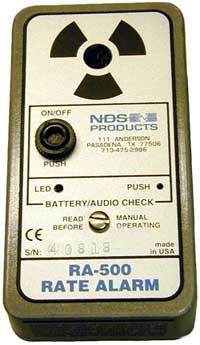
\includegraphics[scale=0.3]{img/alarm.jpg}
  \caption{Akustische Alarmgeräte}
  \label{fig:Alarmgeräte Meter}
\end{figure}
\subsubsection{Film Badges}
Personendosimetrie-Filmabzeichen werden üblicherweise verwendet, um die Strahlenbelastung aufgrund von Gammastrahlen, Röntgenstrahlen und Betateilchen zu messen und aufzuzeichnen. Der Detektor ist, wie der Name schon sagt, ein Stück strahlungsempfindlichen Film. Die Folie ist in einer lichtdichten, dampfdichten Hülle verpackt, die verhindert, dass Licht, Feuchtigkeit oder chemische Dämpfe auf den Film einwirken.
\begin{figure}[htb]
   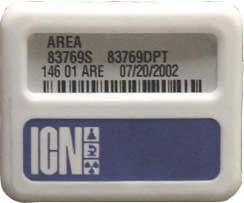
\includegraphics[scale=0.7]{img/area-filmbadge.jpg}
   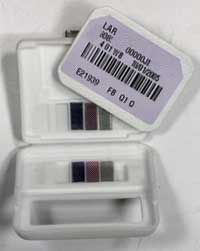
\includegraphics[scale=0.5]{img/FilmBadge.jpg}
  \caption{FilmBadge}
  \label{fig:FilmBadge}
\end{figure}
Es wird ein spezieller Film verwendet, der mit zwei verschiedenen Emulsionen beschichtet ist. Eine Seite ist mit einer großkörnigen, schnellen Emulsion beschichtet, die empfindlich auf geringe Expositionen reagiert. Die andere Seite des Films ist mit einer feinkörnigen, langsamen Emulsion beschichtet, die weniger empfindlich gegenüber Belichtung ist. Wenn die Strahlenexposition dazu führt, dass die schnelle Emulsion in dem verarbeiteten Film zu einem Grad verdunkelt wird, der nicht interpretiert werden kann, wird die schnelle Emulsion entfernt und die Dosis wird unter Verwendung der langsamen Emulsion berechnet.
Der Film ist in einem Filmhalter oder Abzeichen enthalten. Das Abzeichen enthält eine Reihe von Filtern, um die Qualität der Strahlung zu bestimmen. Die Strahlung einer gegebenen Energie wird in unterschiedlichem Maße durch verschiedene Arten von Absorbern abgeschwächt. Daher wird die gleiche Strahlungsmenge, die auf die Plakette auftrifft, unter jedem Filter einen unterschiedlichen Grad an Dunkelfärbung erzeugen. Durch Vergleich dieser Ergebnisse kann die Energie der Strahlung bestimmt und die Dosis berechnet werden, wobei die Filmantwort für diese Energie bekannt ist. Der Ausweishalter enthält außerdem ein offenes Fenster zur Bestimmung der Strahlenbelastung durch Betateilchen. Betateilchen werden effektiv durch eine geringe Menge an Material abgeschirmt.
Die Hauptvorteile eines Filmabzeichens als Personalüberwachungsgerät sind, dass es eine dauerhafte Aufzeichnung bereitstellt, es in der Lage ist, zwischen verschiedenen Energien von Photonen zu unterscheiden, und es Dosen aufgrund verschiedener Arten von Strahlung messen kann. Es ist ziemlich genau für Belichtungen größer als 100 Millirem. 
Die Hauptnachteile bestehen darin, dass sie von einem Prozessor entwickelt und gelesen werden müssen (was zeitaufwendig ist), eine längere Hitzeeinwirkung den Film beeinträchtigen kann und Belichtungen von weniger als 20 Milliram Gammastrahlung nicht genau gemessen werden können.
Filmabzeichen müssen korrekt getragen werden, damit die Dosis, die sie erhalten, genau die Dosis darstellt, die der Träger erhält. Ganzkörper-Abzeichen werden am Körper zwischen Hals und Taille getragen, oft am Gürtel oder an der Hemdtasche. Das Ansteck-Abzeichen wird am häufigsten bei der Röntgen- oder Gammaradiographie getragen. Das Filmabzeichen kann auch beim Arbeiten in einer niedrigen Curie-Quelle getragen werden. Ringabzeichen werden an einem Finger der Hand getragen, der am wahrscheinlichsten ionisierender Strahlung ausgesetzt ist. Ein LIXI-System mit seinem kulminierten und gerichteten Strahl wäre ein Beispiel, bei dem die Überwachung der Hände wichtiger wäre als der gesamte Körper.
\subsubsection{Thermoluminescent Dosimeter (TLD)}
Thermoluminescent Dosimeter(TLD) werden oft anstelle des Filmabzeichens verwendet. Wie ein Filmabzeichen wird es für eine gewisse Zeit (normalerweise 3 Monate oder weniger) getragen und muss dann verarbeitet werden, um die erhaltene Dosis zu bestimmen, falls vorhanden. Thermoluminescent Dosimeter können Dosierungen bis zu 1 Millirem messen, aber unter Routinebedingungen ist ihre niedrige Dosisleistung ungefähr die gleiche wie für Filmabzeichen. TLDs haben eine Genauigkeit von ca. 15\% für niedrige Dosen. Diese Genauigkeit verbessert sich bei hohen Dosen auf etwa 3\%. Die Vorteile einer TLD gegenüber anderen Personalmonitoren sind ihre Linearität der Reaktion auf die Dosis, ihre relative Energieunabhängigkeit und ihre Empfindlichkeit gegenüber niedrigen Dosen. Es ist auch wiederverwendbar, was ein Vorteil gegenüber Filmabzeichen ist. Es wird jedoch keine dauerhafte Aufzeichnung oder Wiederlesbarkeit bereitgestellt, und eine sofortige Auslesung am Arbeitsplatz ist nicht möglich.
\begin{figure}[htb]
\centering
   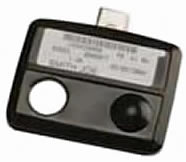
\includegraphics[scale=0.9]{img/TLD.jpg}
  \caption{TLD}
  \label{fig:TLD}
\end{figure}
\subsubsection{Wie es funktioniert}
Eine TLD ist ein Phosphor, wie Lithiumfluorid (LiF) oder Calciumfluorid (CaF), in einer festen Kristallstruktur. Wenn eine TLD ionisierender Strahlung bei Umgebungstemperaturen ausgesetzt wird, wechselwirkt die Strahlung mit dem Phosphorkristall und deponiert die gesamte oder einen Teil der einfallenden Energie in diesem Material. Einige der Atome im Material, die diese Energie absorbieren, werden ionisiert und erzeugen freie Elektronen und Bereiche, denen ein oder mehrere Elektronen fehlen, Löcher genannt. Unvollkommenheiten in der Kristallgitterstruktur wirken als Stellen, an denen freie Elektronen eingeschlossen und an Ort und Stelle arretiert werden können.
Durch Erhitzen des Kristalls vibriert das Kristallgitter, wodurch die eingefangenen Elektronen freigesetzt werden. Freigesetzte Elektronen kehren in den ursprünglichen Grundzustand zurück und geben die eingefangene Energie aus der Ionisation als Licht frei, daher der Name Thermolumineszenz. Freigesetztes Licht wird unter Verwendung von Photovervielfacherröhren gezählt, und die Anzahl der gezählten Photonen ist proportional zu der Strahlungsmenge, die auf den Phosphor trifft.
Anstatt die optische Dichte (Schwärze) eines Films zu lesen, wie es bei Filmabzeichen der Fall ist, wird die Menge an Licht gemessen, die gegenüber dem Erwärmen der einzelnen Stücke des Thermolumineszenzmaterials freigesetzt wird. Die durch diesen Prozess erzeugte "Glühkurve" steht dann in Beziehung zur Strahlenbelastung. Der Prozess kann viele Male wiederholt werden.



























































\chapter{Ergebnisse}
\label{sec:ergebnisse}


\chapter{Diskussion}
\label{sec:diskussion}

\section{Zusammenfassende Bewertung}
\label{sec:überschrift}

\section{Ausblick}
\label{sec:ausblick}

%Literaturverzeichnis
\bibliographystyle{unsrtdin}
\bibliography{Literatur}

\end{document}
